\documentclass[a4paper,11pt,oneside,openany]{jsbook}
%
\usepackage{amsmath,amssymb}
\usepackage{bm}
\usepackage[dvipdfmx,hiresbb]{graphicx}
\usepackage{verbatim}
\usepackage{wrapfig}
\usepackage{ascmac}
\usepackage{makeidx}
%\usepackage[left=37mm, head=30mm, foot=30mm, right=18mm]{geometry}
%
%
\makeindex
%%各種設定いろいろ%
\setlength{\textwidth}{155truemm}      
\setlength{\fullwidth}{\textwidth}    
\setlength{\oddsidemargin}{37truemm}   
\addtolength{\oddsidemargin}{-1truein} 
\setlength{\topmargin}{30truemm}      
\setlength{\textheight}{237truemm}    
\addtolength{\topmargin}{-1truein}
\makeatother
%
% 
\def\linesparpage#1{\baselineskip=\textheight
   \divide\baselineskip by #1}
\def\kcharparline#1{
   \ifx\xkanjiskip\undefined
   \jintercharskip 0mm plus 0.2mm minus 0.2mm
   \else
   \xkanjiskip 0mm plus 0.2mm minus 0.2mm
   \fi
   \settowidth{\textwidth}{}
   \multiply\textwidth by #1
   }

%%%%%%%%%%ここから
\begin{document}
\linesparpage{32} 
\kcharparline{40}

%%% title.tex読み込み
\begin{titlepage}
\begin{flushright}
{\large
指導教員(主査):牛尼 剛聡 准教授 \\ % 主査
副査:上岡 玲子 准教授             \\ % 副査
副査:森本 有紀 助教
}
\end{flushright}
\begin{center}
\vspace*{120truept}
{\huge 修 士 論 文}\\ 
\vspace{30truept}
{\Large レビューへのフィードバックに基づいたアイテムの絞り込みと品定めの支援に関する研究}\\ % タイトル
\vspace{10truept}
{\large A Study for Supporting Item Selection Using Feedback on Reviews}\\ % 英語タイトル
\vspace{140truept}
{\Large 九州大学大学院芸術工学府 芸術工学専攻 コンテンツクリエーティブデザイン}\\ % 所属
{\Large 平成28年4月入学 学籍番号 2DS16081W}\\ % 学籍番号
\vspace{10truept}
{\Large 南 大智}\\ % 著者
\vspace{50truept}
{\Large 2018年1月提出}\\ % 提出日
\end{center}
\end{titlepage}

\frontmatter

\chapter{要旨}
現在,世界中には莫大な数のアイテムが存在しており,ユーザは自分の好みに合ったアイテムを発見することが困難になっている.こうした中で,アイテムに対するレビューを閲覧可能な投稿型レビューサイトの役割が重要になっている.しかし,レビューを投稿した全てのレビュワーが信頼できるとは限らない.中には,悪意を持ったレビュワーや対象ユーザから見て信頼に値しないレビュワーも存在する.ユーザがオンラインレビューサイト上でアイテム選別を行う際に,見知らぬレビュワーが信頼できるかどうかを判断することは困難である.また,信頼に値しないレビュワーの存在が,アイテム選別の妨げになる場合も考えられる.本研究では,対象ユーザに関する既知の情報を用いて,未知のレビュワーに対する信頼を予測するモデルを提案する.提案モデルに基づき,投稿型レビューサイトにおけるレビュワーへの信頼の予測を行い,得られた信頼情報を用いて,アイテム選別の支援を行う.私たちは,「莫大な数のアイテムの中からの絞り込み」と「候補アイテムに対する価値判断(品定め)」のそれぞれにおける支援のアプローチを提案し,実装したプロトタイプを用いて被験者実験を行なった.
\par


\tableofcontents

\mainmatter

%%% はじめに
\chapter{はじめに}
	\section{研究の背景}
近年,インターネットの普及に伴い,商品の購入や調査などがインターネットを介して行われることが一般的になった.また,インターネット上に存在するアイテムの数も増加している.例えば,2017年3月の時点で,日本における代表的なECサイト「楽天市場」\cite{rakuten}には194,023,903点の商品が存在する\cite{rakuten_info}.また,特定のカテゴリのアイテムも莫大な数が存在し,Google Booksでは,2010年8月5日時点での書籍総数は1億2986万4880冊としている\cite{google}.このような「情報過多」\cite{info}の中で,ユーザは自分の好みに合うアイテムを探さなければならない.
\par
一方で,特定の分野における商品のレビューを集めたSNS形式のWebサイト(オンラインレビューサイト)が多くのユーザを獲得している.日本におけるオンラインレビューサイトの代表例として,化粧品に対するレビューを集めた「@cosme」(アットコスメ)\cite{@cosme},書籍を対象とした「読書メーター」\cite{bookmeter},映画を対象とした「Yahoo!映画」\cite{yahoo}などがあげられる.レビューはアイテムの選別を行う上で非常に有用であり,株式会社情報通信総合研究所の調査\cite{ict}では,インターネットショッピングサービスを利用する際に,全体の74.8%の人がレビューを参考にすると回答している.投稿されているレビューには,利用者の実際の経験に基づく感想や説明が書かれており,ユーザはアイテムが自分にとって価値があるかどうかについて,購入する前に判断することができる.
\par
また,オンラインレビューサイトでは,ユーザが指定したアイテムのレビューを表示するだけでなく,レビューを利用したアイテム推薦機能も提供されている場合が多い.情報推薦の方式には,一般的に,コンテンツに基づくフィルタリング(content-based filtering)と,協調フィルタリング(collaborative filtering)の2種類がある\cite{hijikata2}.例えば,「読書メーター」においては,「この本を読んだ人はこんな本も読んでいます」という協調フィルタリングを用いた書籍推薦機能を提供している.「読書メーター」では,ユーザが読んだ書籍を登録できるため,登録データの分析によって求められるユーザ同士の類似性を基にして書籍の類似性を推定し,ユーザが興味を持った書籍に基づいて,そのユーザが興味を持つ可能性が高いと考えられる書籍を推薦する.
\par
一般的に,オンラインレビューサイトにおいて,レビューの価値は等価に扱われている.しかし,投稿されているレビューは対象ユーザにとって役に立つレビューばかりではなく,中には対象ユーザにとって役に立たないレビューも存在する場合がある.例えば、図に示すような,悪意のあるユーザや業者によるスパムレビューがECサイトやオンラインレビューサイト上には存在する.スパムレビューはアイテムの価値を判断する上で問題がある.また,ユーザによって好ましくないレビューも存在する.


	\section{研究の目的}
従来では,レビューの価値は等価に扱われていた.本研究では,レビューの価値はユーザによって異なるという仮定に基づいて,より効率的なアイテム選別の支援を行う.以下の2つのアプローチでアイテム選別の支援を行う
\par
\subsection{協調フィルタリングによるアイテムの絞り込み}
協調フィルタリングは,ユーザの過去の履歴を見て, 対象ユーザと同じアイテムを多く選択しているユーザは嗜好が類似していると判断し,類似ユーザが選択・購入したアイテムを推薦することで,高い精度をもった推薦が行える有効な手法である.
例えば,図\ref{fig:kyocho}では,対象ユーザが書籍Bを読んだことがあり,それ以外の書籍は未読である状況だとする.対象ユーザ以外で,書籍Bを読んでいる二人のユーザは,それぞれ書籍Aと書籍Cを読んでいるので,対象ユーザには書籍Aと書籍Cを推薦するという仕組みである.
\begin{figure}[htb]
	\begin{center} %貼り付ける位置指定
		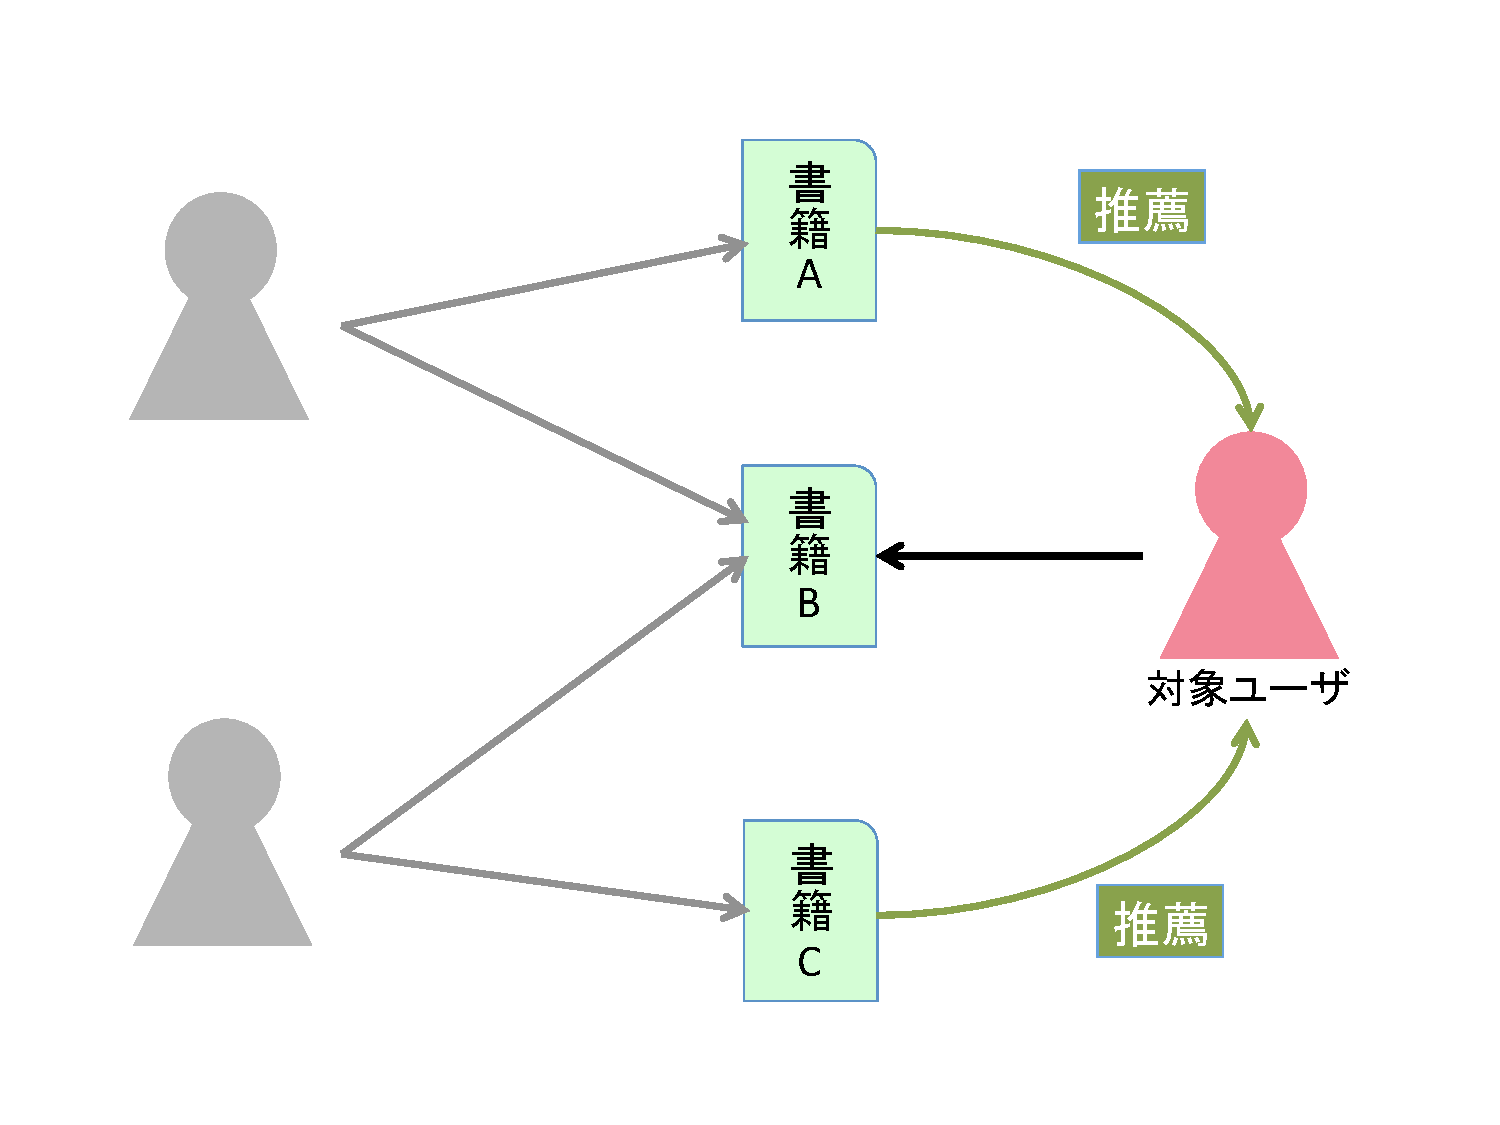
\includegraphics[width = 100mm]{figures/kyocho.pdf} %貼り付ける画像と大きさ
	\end{center}
	\caption{一般的な協調フィルタリングによる推薦} %キャプション
	\label{fig:kyocho} %TEXコード内で使う変数指定
\end{figure}
\par
上記の書籍推薦機能で用いられている協調フィルタリングは一般的に.「同一の書籍を読んだユーザ同士は書籍選択における嗜好が似ている」という仮定に基づいて推薦を行っている.しかし,書籍をはじめ,さまざまな物事を見たり考えたりするとき,人はそれぞれの立場から評価や考察を行う.書籍を対象としたオンラインレビューサイトにおいては,同一書籍に対するレビューであっても,各レビュワーのレビューにおける評価の視点に違いが見られる場合が多い.例えば,漫画書籍に対するレビューの場合,絵についての評価をするレビュワーもいれば,ストーリーについての評価をするレビュワーもいる.さまざまな内容のレビューの中で,どのレビューに対して共感できるかどうかは,ユーザによって違いがあることが考えられ,同一アイテムを選択したユーザ同士であっても,嗜好の類似性が低い場合がある.そこで,書籍を対象としたオンラインレビューサイトにおける協調フィルタリングを利用した書籍情報の推薦の際に,対象ユーザのレビュワーに対する好みに基づいて,レビュワーの重みを変更して推薦書籍の計算を行うことで,推薦精度を向上させる.
\subsection{レビュー推薦によるアイテムの品定め}
次に,アイテム推薦により,選択候補のアイテムが絞り込まれた後,ユーザはアイテムが本当に自分の好みに合うかどうかについて,価値を判断する(品定め)行為を行うことが考えられる.ユーザが未知のアイテムの品定めを行う際に,アイテムに対する感想や説明が書かれている口コミ情報,すなわちレビューは有用な情報である.しかし,オンラインレビューサイトに投稿されているレビューの数は莫大であるため,効率的にレビューを閲覧することは難しいという問題がある.また,投稿されているレビューは対象ユーザにとって役に立つレビューばかりではなく,中には対象ユーザにとって役に立たないレビューも存在する.そこで,オンラインレビューサイトにおける協調フィルタリングによる推薦アイテムを品定めする際,ユーザが品定めしやすいようにレビューを並び替えることによって,効率的な品定めの支援を行う.
\par
本研究では,レビューに対するフィードバックを基に,推定した対象ユーザのレビュワーに対する信頼度を用いて,アイテム選別の支援を行う.具体的には,アイテムの「絞り込み」と「品定め」の2つの行為に着目し,それぞれにおける評価実験を行う.

	\section{論文の構成}
本論文の構成を以下に示す.本章では,本研究の背景および目的について説明した.第2章では,本研究に関連する研究を紹介し,本研究の独自性について述べる.第3章では,レビューに対するフィードバックに基づくレビュワーの信頼推定手法について述べる.第4章では,アイテムの絞り込みのために,第3章で推定された信頼情報を用いた協調フィルリング手法について説明し,評価実験の結果,考察について述べる.第5章では,アイテムの品定め支援のために,信頼情報を用いたレビュー推薦手法について説明し,評価実験の結果,考察を述べる.第6章では,今後の課題と展望を示し,本論文の総括を行う.



\chapter{関連研究}
	\section{情報推薦におけるフィードバックの活用}
\label{sec:related_feed}
情報検索において,ユーザがクエリを正しく指定することができない場合に要求する情報を取得できないことは,重要な問題として認識されてきた. これを解決する代表的な手法として, 適合フィードバックが知られている\cite{feedback}.適合フィードバックは,情報検索において検索結果として出力された文章の内容に対するユーザの反応に基づいて,検索質問や検索戦略,検索式を修正する手法である\cite{hijikata}.このとき,クエリを修正する基となるのは,文書自体に対してのフィードバックである.
代表的なクエリの修正は,Rocchioのアルゴリズムが用いられることが多く,次のように定義される.
\begin{equation}
\mathbf{q_m} = \alpha\mathbf{q_0}+\frac{\beta}{|D_R|}\sum_{\mathbf{d_i}\in{D_R}}{\mathbf{d_i}}-\frac{\gamma}{|D_N|}\sum_{\mathbf{d_i}\in{D_N}}{\mathbf{d_i}}
\end{equation}
\par
ここで,$D_R$と$D_N$は,それぞれユーザに与えられた検索結果のうち,興味のあるとした文書,興味がないとした文書である.また,$\alpha$,$\beta$,$\gamma$はそれぞれ元のクエリベクトル,正の影響ベクトル,負の影響ベクトルにどれくらいの重みを与えるかを決めるパラメータである.推薦するコンテンツの種類がテキストである場合は,ベクトルはキーワードの出現頻度で表され,tf・idf法などを用いて,キーワードに重みを付ける方法が適用される.
\par
このように,推薦コンテンツ自体に対するフィードバックを利用する研究として,例えば,顔らは,スマートフォンでの効率的な商品選別を行うために,ユーザの振る舞いを基にした適合フィードバックを用いて推薦の最適化を行う手法を提案している\cite{yan}.
\par
一般的に,適合フィードバックは,対象とするアイテム自体にフィードバックを与え,結果を最適化する手法である.それに対して,本研究では対象となるアイテムである書籍自体ではなく,書籍に関するレビューに対するフィードバックをを与えるという点で独自性がある.

	\section{レビューの品質推定}
Amazonでは,レビューが役に立ったかについての投票ボタンを設置しており,投票に基づいてレビューの品質を決定している.しかし,Amazonのレビュー全体のうち約10%程度しか評価されていない\cite{amazon}.また,古いレビューは多くの投票を集め、上位に表示されるが、まだ票を持っていない新しいレビューは役に立たないと考えられている\cite{Moghaddam}.また,多くのポジティブな投票を得たレビューは、より多くのポジティブな投票を集めやすい.これらの問題を解決するために,レビューの品質スコアを推定する研究が行われている\cite{Raghavan}.
また,レビューなどのテキスト情報の信頼性に関して,さまざまな研究が行われてきた\cite{iki,muk,xie,wang}.これらの研究では,スパムなど,不当なレビューの投稿を行う悪意を持った投稿者を問題視しており,「スパムであるか否か」「虚偽の投稿であるか否か」ということに関する議論を展開している.
レビューのランキングやフィルタリングに関する研究は,レビューの客観的な価値に関するものが多く,「対象ユーザにとって有益であるか」や「対象ユーザが好感を抱くか」など,レビューに対する個人的な嗜好についてはあまり議論されていない.本研究においては,個人的な観点からのレビューの価値について着目する.

	\section{レビューを利用した情報推薦}
近年,レビューを利用した情報推薦に関する研究は多く行われている.レビューを利用した推薦の方向性として主に以下の3点がある\cite{Li}.
\begin{itemize}
 \item ユーザの好みに関する情報を抽出することでデータの希薄さの問題に対応する.
 \item コールドスタート問題に対応する.
 \item ユーザのコンテキストや潜在的な嗜好因子など評価値以外の推薦に有用な情報をレビューから導出する.
\end{itemize}
\par
レビューを利用してユーザの嗜好を抽出し情報推薦を行う研究として,林ら\cite{hayashi}はユーザが書いたレビューからユーザの嗜好として興味語とその極性を抽出し,興味語が含まれ極性が一致するレビューをもつ映画を推薦することで,ユーザの好みに合った推薦が可能であることを示した.
\par
一般的に,上記のような情報推薦に関する研究は,アイテムの効率的な選別を支援するためにアイテムを推薦し,推薦アイテムがどれだけ対象ユーザの好みに合っているかという点を評価しているが,アイテムを推薦した後の価値判断の支援は行っていない.本研究では,推薦アイテムが提示された後に,ユーザが行うと予想される品定め行為を支援することで,アイテムの効率的な選別を支援する.
また,ユーザが過去に選択したアイテム全てに対してレビューを入力させることでユーザの嗜好を獲得するアプローチは,ユーザへの負担が大きいという点で現実的ではない.そこで,本研究ではアイテムのレビューに対するフィードバックを用いて,間接的に,ユーザの嗜好を推定するアプローチをとる.

	\section{協調フィルタリング拡張手法}
協調フィルタリングを拡張する手法に関して,今までにさまざまな提案がされてきた.協調フィルタリングでは,ユーザのアイテムに対する評価値データを基にして推薦を行うが,評価値の欠損により推薦が上手く行えないというスパース性の問題に対して,少ない評価値情報から効率的に未知の評価値を推定する手法として,Matrix Factorization(MF)\cite{MF}が有効であることが確認されている.MFは,次元削減を行うことで,ユーザの潜在的特徴を利用し,より疎な部分が少ない評価値行列を作成することで,精度の良い推薦を行うことができる.また,ユーザやアイテムの潜在的特徴に関して,評価値以外の情報を利用する手法についても研究されている.協調フィルタリングとコンテンツに基づくフィルタリングを混合させたモデルであるコンテンツブーステッド協調フィルタリング\cite{Melville}においては,ナイーブベイズ法を用いて,ユーザの属性(年齢や性別など)からユーザアイテムマトリックスの欠損値を補完して,擬似マトリックスを生成する.また近年では,潜在的特徴の解析手法として近年注目されているトピックモデルを協調フィルタリングに用いた研究も行われており,代表的な手法としてLDAの著者であるBleiらが提案したCTRが知られている\cite{CTR}.CTRは,アイテムに関するテキスト情報からトピックを抽出して,ユーザとアイテムの特徴ベクトルに反映させることで,評価値が存在しないアイテムであってもトピック情報を基に評価値を推定する手法である.これらの手法では,いずれもユーザの潜在的特徴を用いて評価値の推定を行っているが,評価における観点は考慮されていない.
\par
本研究における評価観点を推定するためには,ユーザの書籍に対する印象を知る必要がある.
GroupLens\cite{grouplens}においてはユーザのアイテムに対する評価を明示的に入力させるが,ユーザが過去に選択したアイテム全てに対してレビューを入力させることでユーザの嗜好を獲得するアプローチは,ユーザへの負担が大きいという点で現実的ではない.そこで,本研究ではアイテムのレビューに対するフィードバックを用いて,間接的に,ユーザの嗜好を推定するアプローチをとる.


\chapter{レビューへのフィードバックによるレビュワーの信頼推定}
本論文では,対象ユーザが既知のレビュワーに対する信頼度に基づいて,未知のレビュワーに対する信頼度を予測するモデルを提案する.提案モデルでは,対象ユーザは既知であるユーザに対する信頼度の評価を入力する.評価されたユーザの特徴と未知のユーザの特徴との間の類似度を求めることで未知のユーザに対する信頼度を推定する.

	\section{レビューへの評価入力インターフェース}
\label{sec:feedback}
図\ref{fig:feedback_image}は,オンラインレビューサイトにおけるレビューに対する評価の入力インターフェースの例を表す.対象ユーザはこのインターフェースを用いて,既知のユーザに対する評価を入力する.この図においては,レビュー文の右下に表示されている二つのアイコンが評価の入力ボタンであり,支持と書いてあるアイコンはポジティブな評価,不支持と書いてあるアイコンはネガティブな評価を入力するために利用する.また,レビューに対する評価がどちらとも言えない場合は,どちらのアイコンもクリックしないことで,中立の表現とする.システムはユーザから入力された各レビューへの評価を,ユーザプロファイル情報として登録する.

\begin{figure}[tb]
	\begin{center} %貼り付ける位置指定
		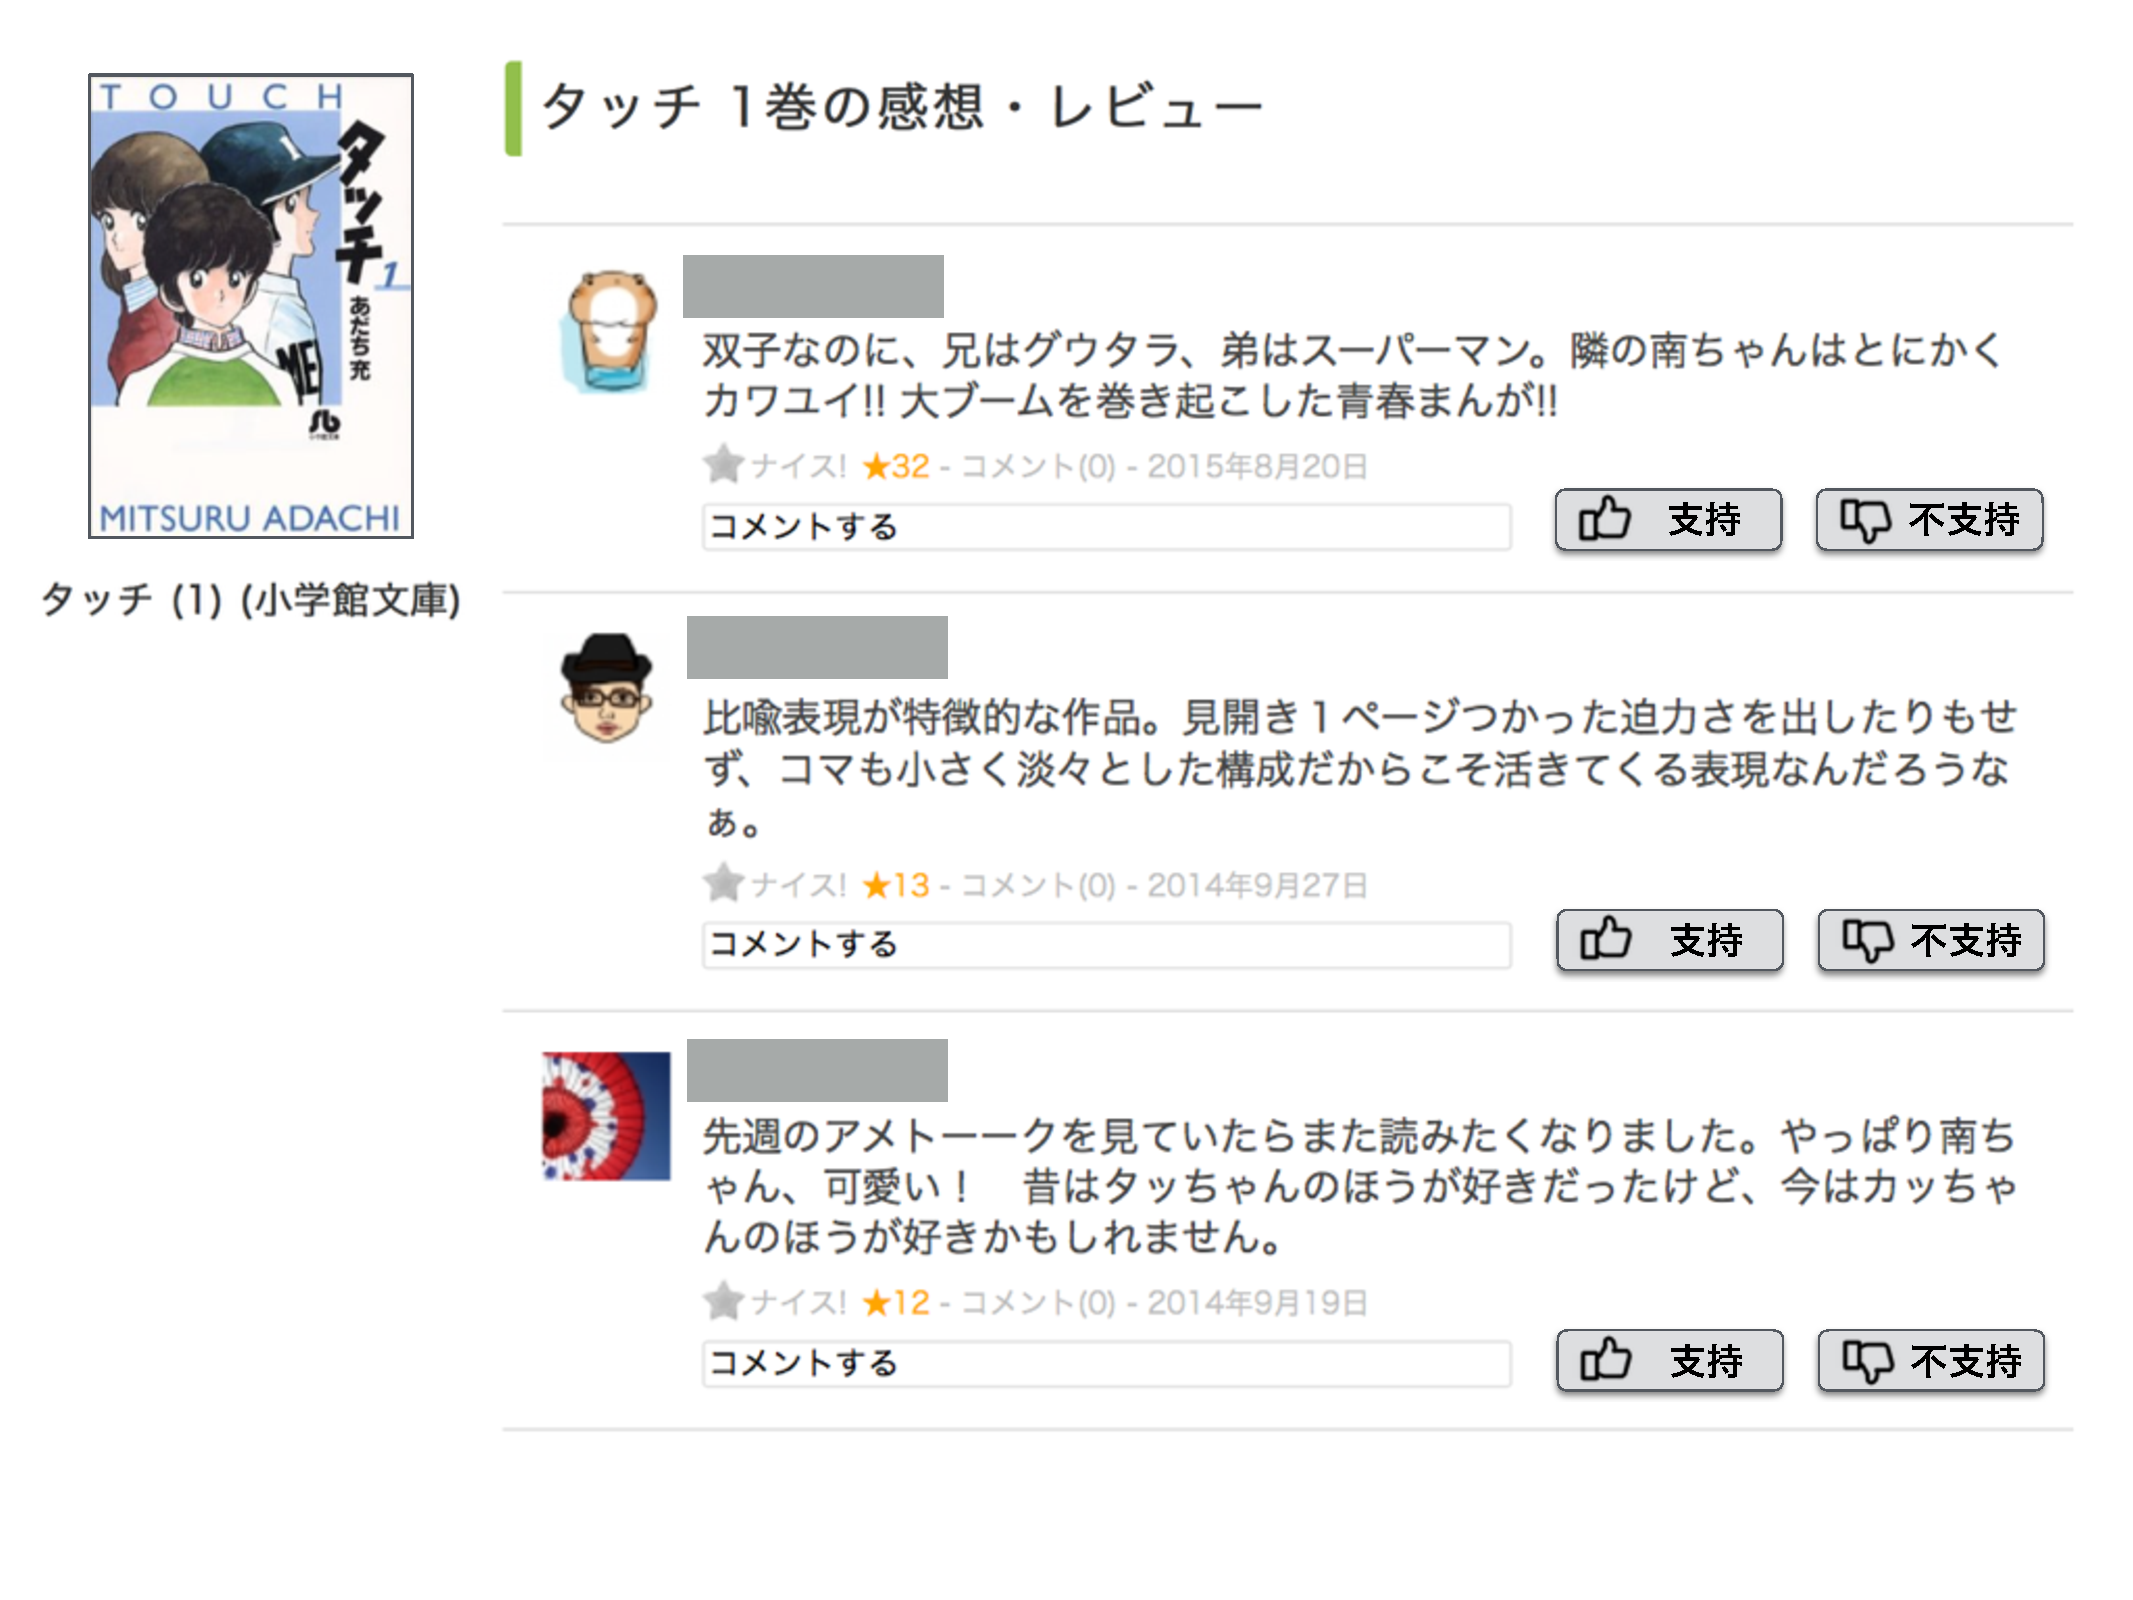
\includegraphics[width = 110mm]{figures/feedback_image.pdf} %貼り付ける画像と大きさ
	\end{center}
	\caption{インターフェース上での評価の入力例} %キャプション
	\label{fig:feedback_image} %TEXコード内で使う変数指定
\end{figure}




\chapter{レビュワーの信頼度に基づくアイテムの絞り込み支援}
	\section{評価の観点の違いを考慮したレビュワーの重み付け}
\subsection{アイテム推薦における評価観点情報の活用}
協調フィルタリングは一般的に.「同一の書籍を読んだユーザ同士は書籍選択における嗜好が似ている」という仮定に基づいて推薦を行っている.しかし,書籍をはじめ,さまざまな物事を見たり考えたりするとき,人はそれぞれの立場から評価や考察を行う.例えば,漫画書籍の場合,絵が美しい漫画を好む人は,「絵が美しいかどうか」が漫画を評価する上での重要な要素だと考え,ストーリーが面白い漫画を好む人は,「ストーリーが面白いかどうか」が漫画を評価する上での重要な要素だと考える場合がある.協調フィルタリングにおいて,このようなユーザの評価における観点を考慮しないことによって,ユーザの嗜好に合わないアイテムが推薦される可能性がある.例えば,アイテム$i$に対して,$A$という観点からの特徴を好んで選択したユーザ集合$U_A$と,アイテム$i$に対して,$B$という観点からの特徴を好んで選択したユーザ集合$U_B$が存在するとする.対象ユーザがアイテム$i$を選択したとき,一般的な協調フィルタリングでは$U_A$と$U_B$は対象ユーザと同じアイテムを選択しているため,嗜好が類似していると判断される.しかし,対象ユーザがアイテム$i$を観点$A$からの特徴に基づいて選択していた場合,$U_A$は対象ユーザとの嗜好の類似性が高いと言えるが,$U_B$は$U_A$と比べると,対象ユーザとの嗜好の類似性は低いと考えられる.つまり,このような場合であれば,$U_B$に基づいて推薦されるアイテムは,対象ユーザの嗜好に合わない可能性があるという問題点がある.
\par
本節では,オンラインレビューサイトにおける協調フィルタリングを利用したアイテム推薦の際に,対象ユーザの評価観点を考慮し,対象ユーザが支持する評価観点とレビュワーの評価観点の類似性に基づいて書籍推薦を行うことで,推薦精度を向上させる手法を提案する.書籍を対象としたオンラインレビューサイトにおいては,同一書籍に対するレビューであっても,各レビュワーのレビューにおける評価の観点に違いが見られる場合が多い.例えば,漫画書籍に対するレビューの場合,絵についての評価をするレビュワーもいれば,ストーリーについての評価をするレビュワーもいる.このようなレビューの観点の違いを解析することによって,評価観点を推定できると考えられる.レビュワーの評価観点の計算には,Latent Dirichlet Allocation(LDA)\cite{Blei}を用いる.具体的には,書籍を評価するための代表的なトピックを学習し,学習したトピックモデルを用いて,対象とするレビュワーのレビューはどのトピックが生成しやすいかについて推論計算することで求められる多項分布をレビュワーの評価観点とする.
\subsection{システムの概要}
本論文では,書籍を対象としたオンラインレビューサイトにおいて,ユーザが書評レビューに対する評価をフィードバックとして与えることで,推薦の内容を最適化してユーザに再提示するシステムを提案する.図\ref{fig:sys}に本システムの概要を示す.
\begin{figure}[tb]
\begin{center}
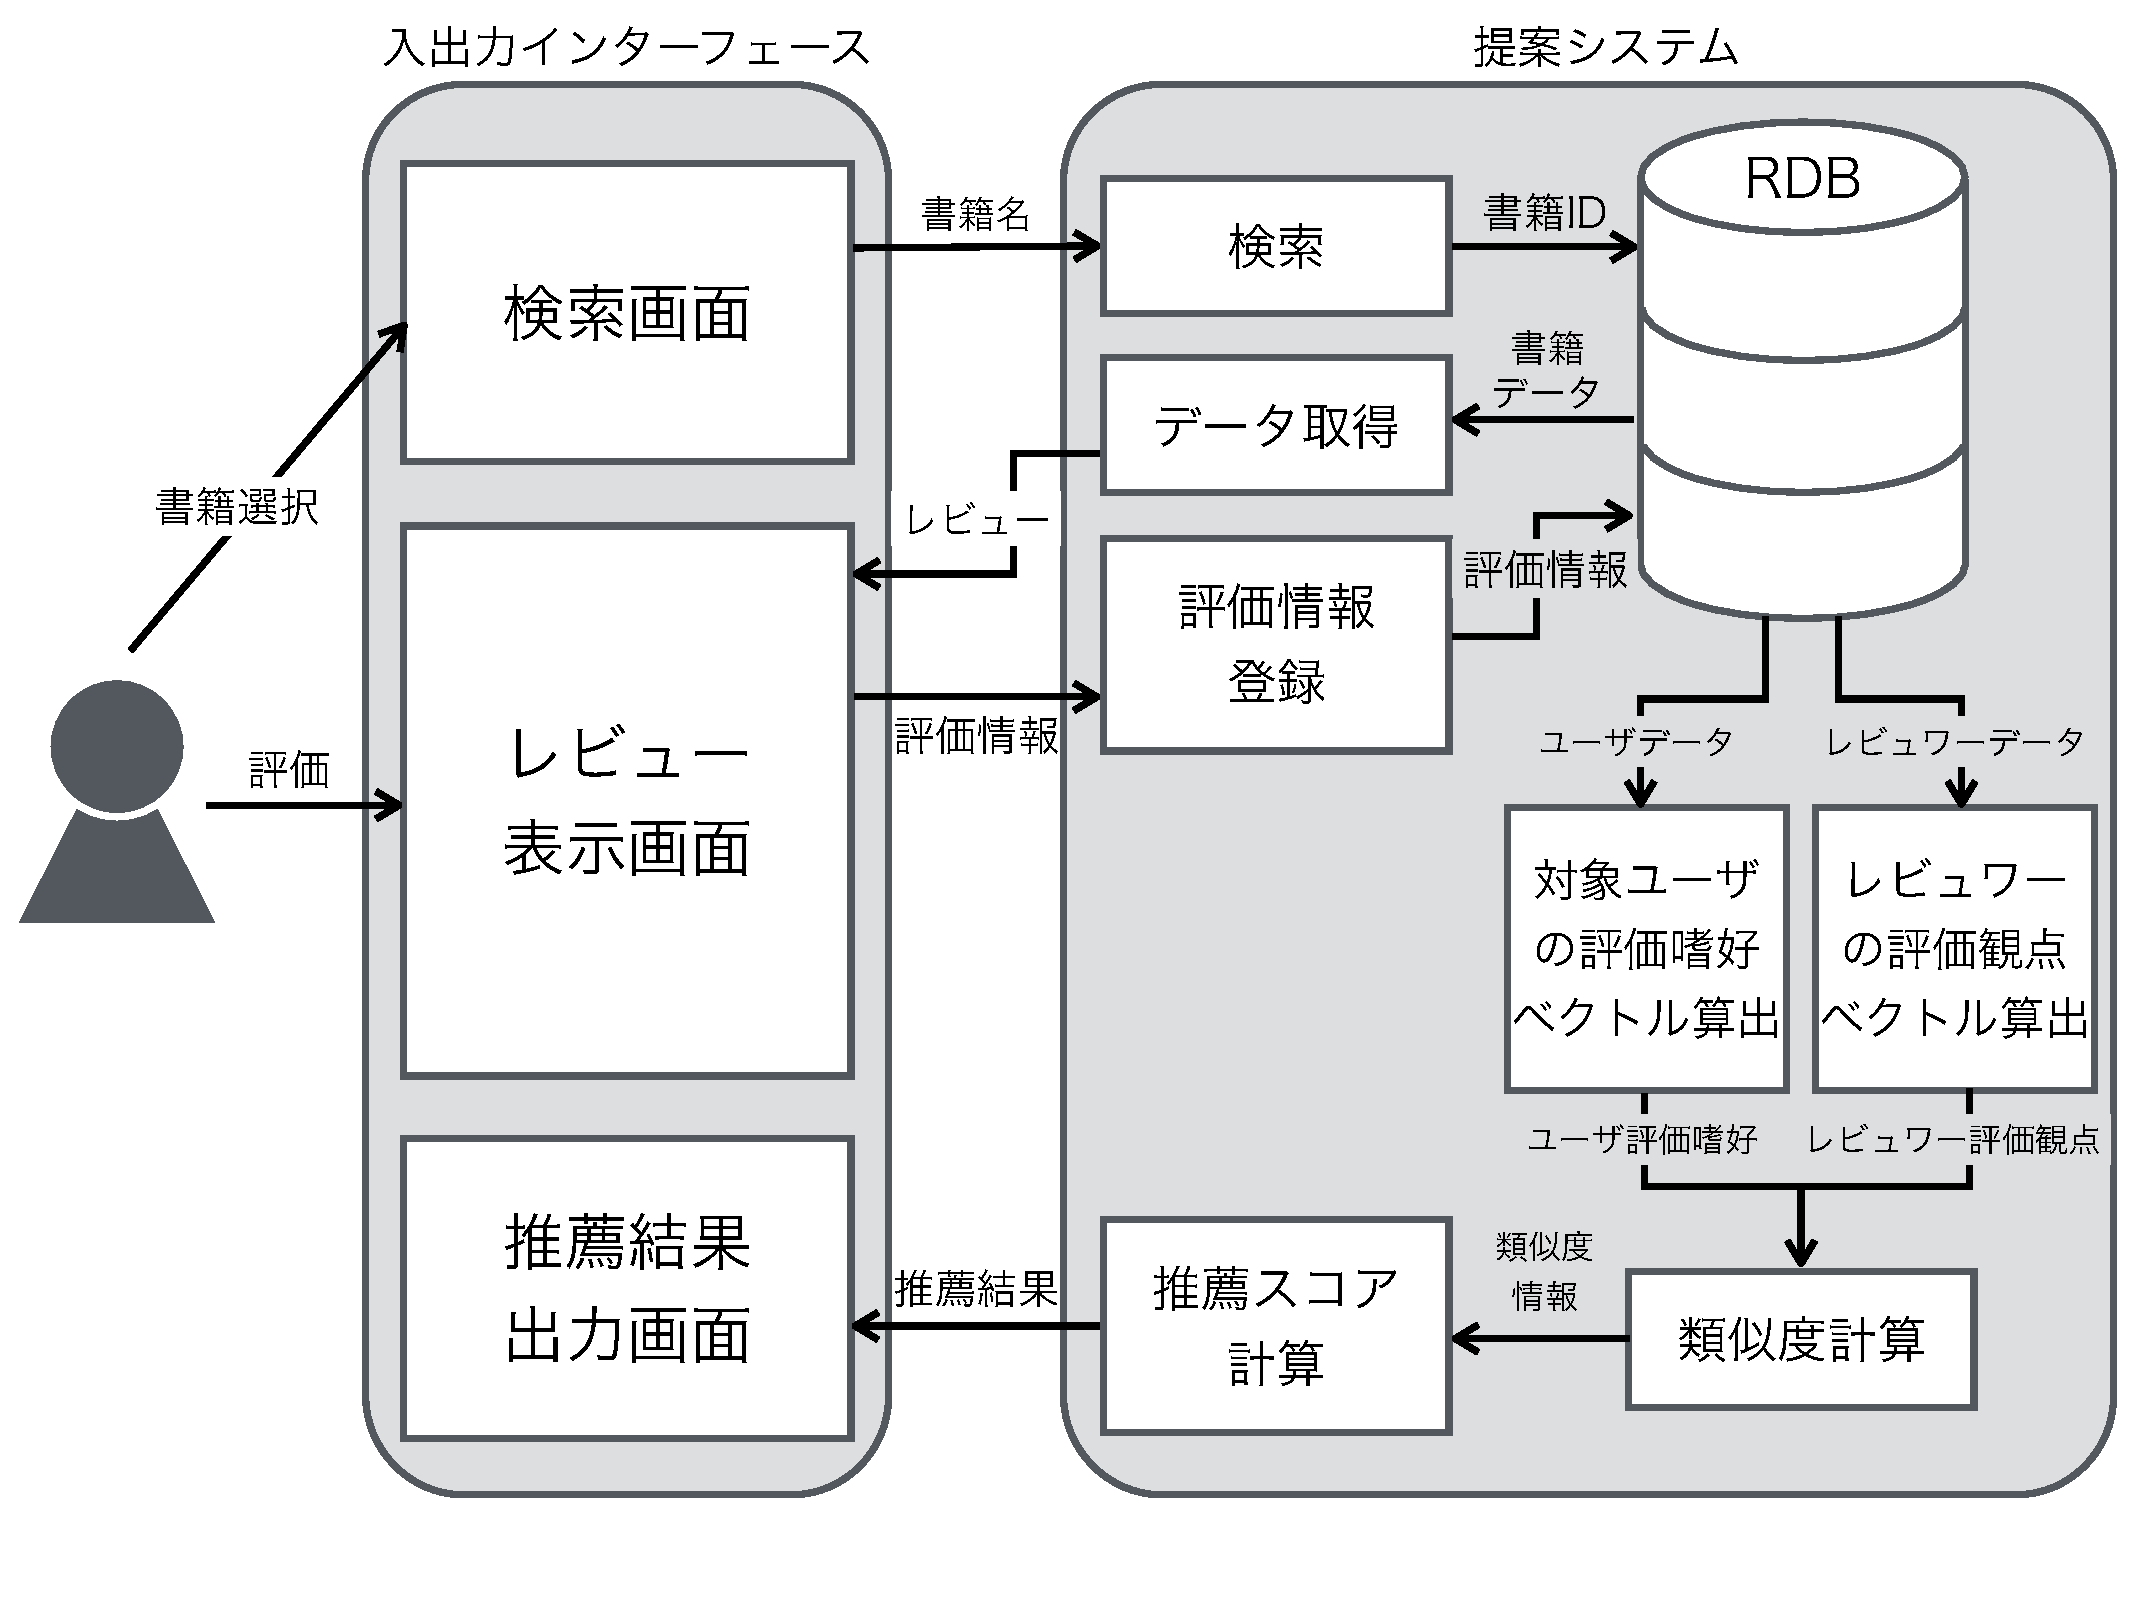
\includegraphics[width = 70mm]{figures/sys_image.pdf}
\end{center}
\caption{システムの概要}
\label{fig:sys}
\end{figure}
本システムでは,対象ユーザが選択した書籍に関するページにおいて,その書籍に対するレビュー,推薦書籍を表示する.推薦書籍の初期値は各ユーザの重要度は均一として一般的な協調フィルタリング手法に基づいて求める.対象ユーザはレビューを読み,個々のレビューに対して支持するかどうかについての評価を支持・不支持・中立のどれかとして入力する.評価されたレビュー集合を解析することで,対象ユーザの評価嗜好を求める.レビュワーの評価観点は,あらかじめLDAを用いて学習した,書籍を評価するためのトピックに対する分布を推論計算することで求める.そして,対象ユーザの評価嗜好と各レビュワーの評価観点との間のコサイン相関値を求め,その値をレビュワーに対する重みとして,推薦書籍の再計算および再提示を行う.
\subsection{LDAを用いた評価観点の解析}
		\subsubsection{Latent Dirichlet Allocation(LDA)}
LDAとは,Bleiらが提案したトピックモデルである.トピックモデルとは,1つの文書が1つまたは複数のトピックをもつと仮定し,文書ごとのトピック分布$\theta_{d} = (\theta_{d1},...,\theta_{dK})$と,それらのトピックごとの単語分布$\phi_{z} = (\phi_{z1},...,\phi_{zN})$に基づいて確率的に文書を生成するモデルである.ここで,$\theta_{dz} = p(z|\theta_{d})$は文書$d$にトピック$z$が割り当てられる確率で,$\phi_{zw} = p(w|\phi_{z})$はトピック$z$で単語wが生成される確率である.具体的な文書の生成は次のように行われる.
\begin{enumerate}
\item For トピック$z = 1, ... , K$
	\begin{enumerate}
	\setlength{\itemindent}{2cm}
 	\item 単語分布を生成 $\phi_{z} 〜 ディリクレ分布(\beta)$
	\end{enumerate}
\item For 文書$d = 1, ... ,D$
	\begin{enumerate}
	\setlength{\itemindent}{2cm}
 	\item トピック分布を生成 $\theta_{d} 〜 ディリクレ分布(\alpha)$
	\setlength{\itemindent}{2cm}
 	\item For 単語$w = 1, ... ,N$
		\begin{enumerate}
		\setlength{\itemindent}{3cm}
		\item トピックを生成 $z_{dw} 〜 多項分布(\theta_{d})$
		\setlength{\itemindent}{3cm}
		\item 単語を生成 $w_{dw} 〜 多項分布(\phi_{z_{dw}})$
		\end{enumerate}
	\end{enumerate}


\end{enumerate}

この生成過程を表すグラフィカルモデルは図\ref{fig:lda}のように表される.
\begin{figure}[tb]
	\begin{center} %貼り付ける位置指定
		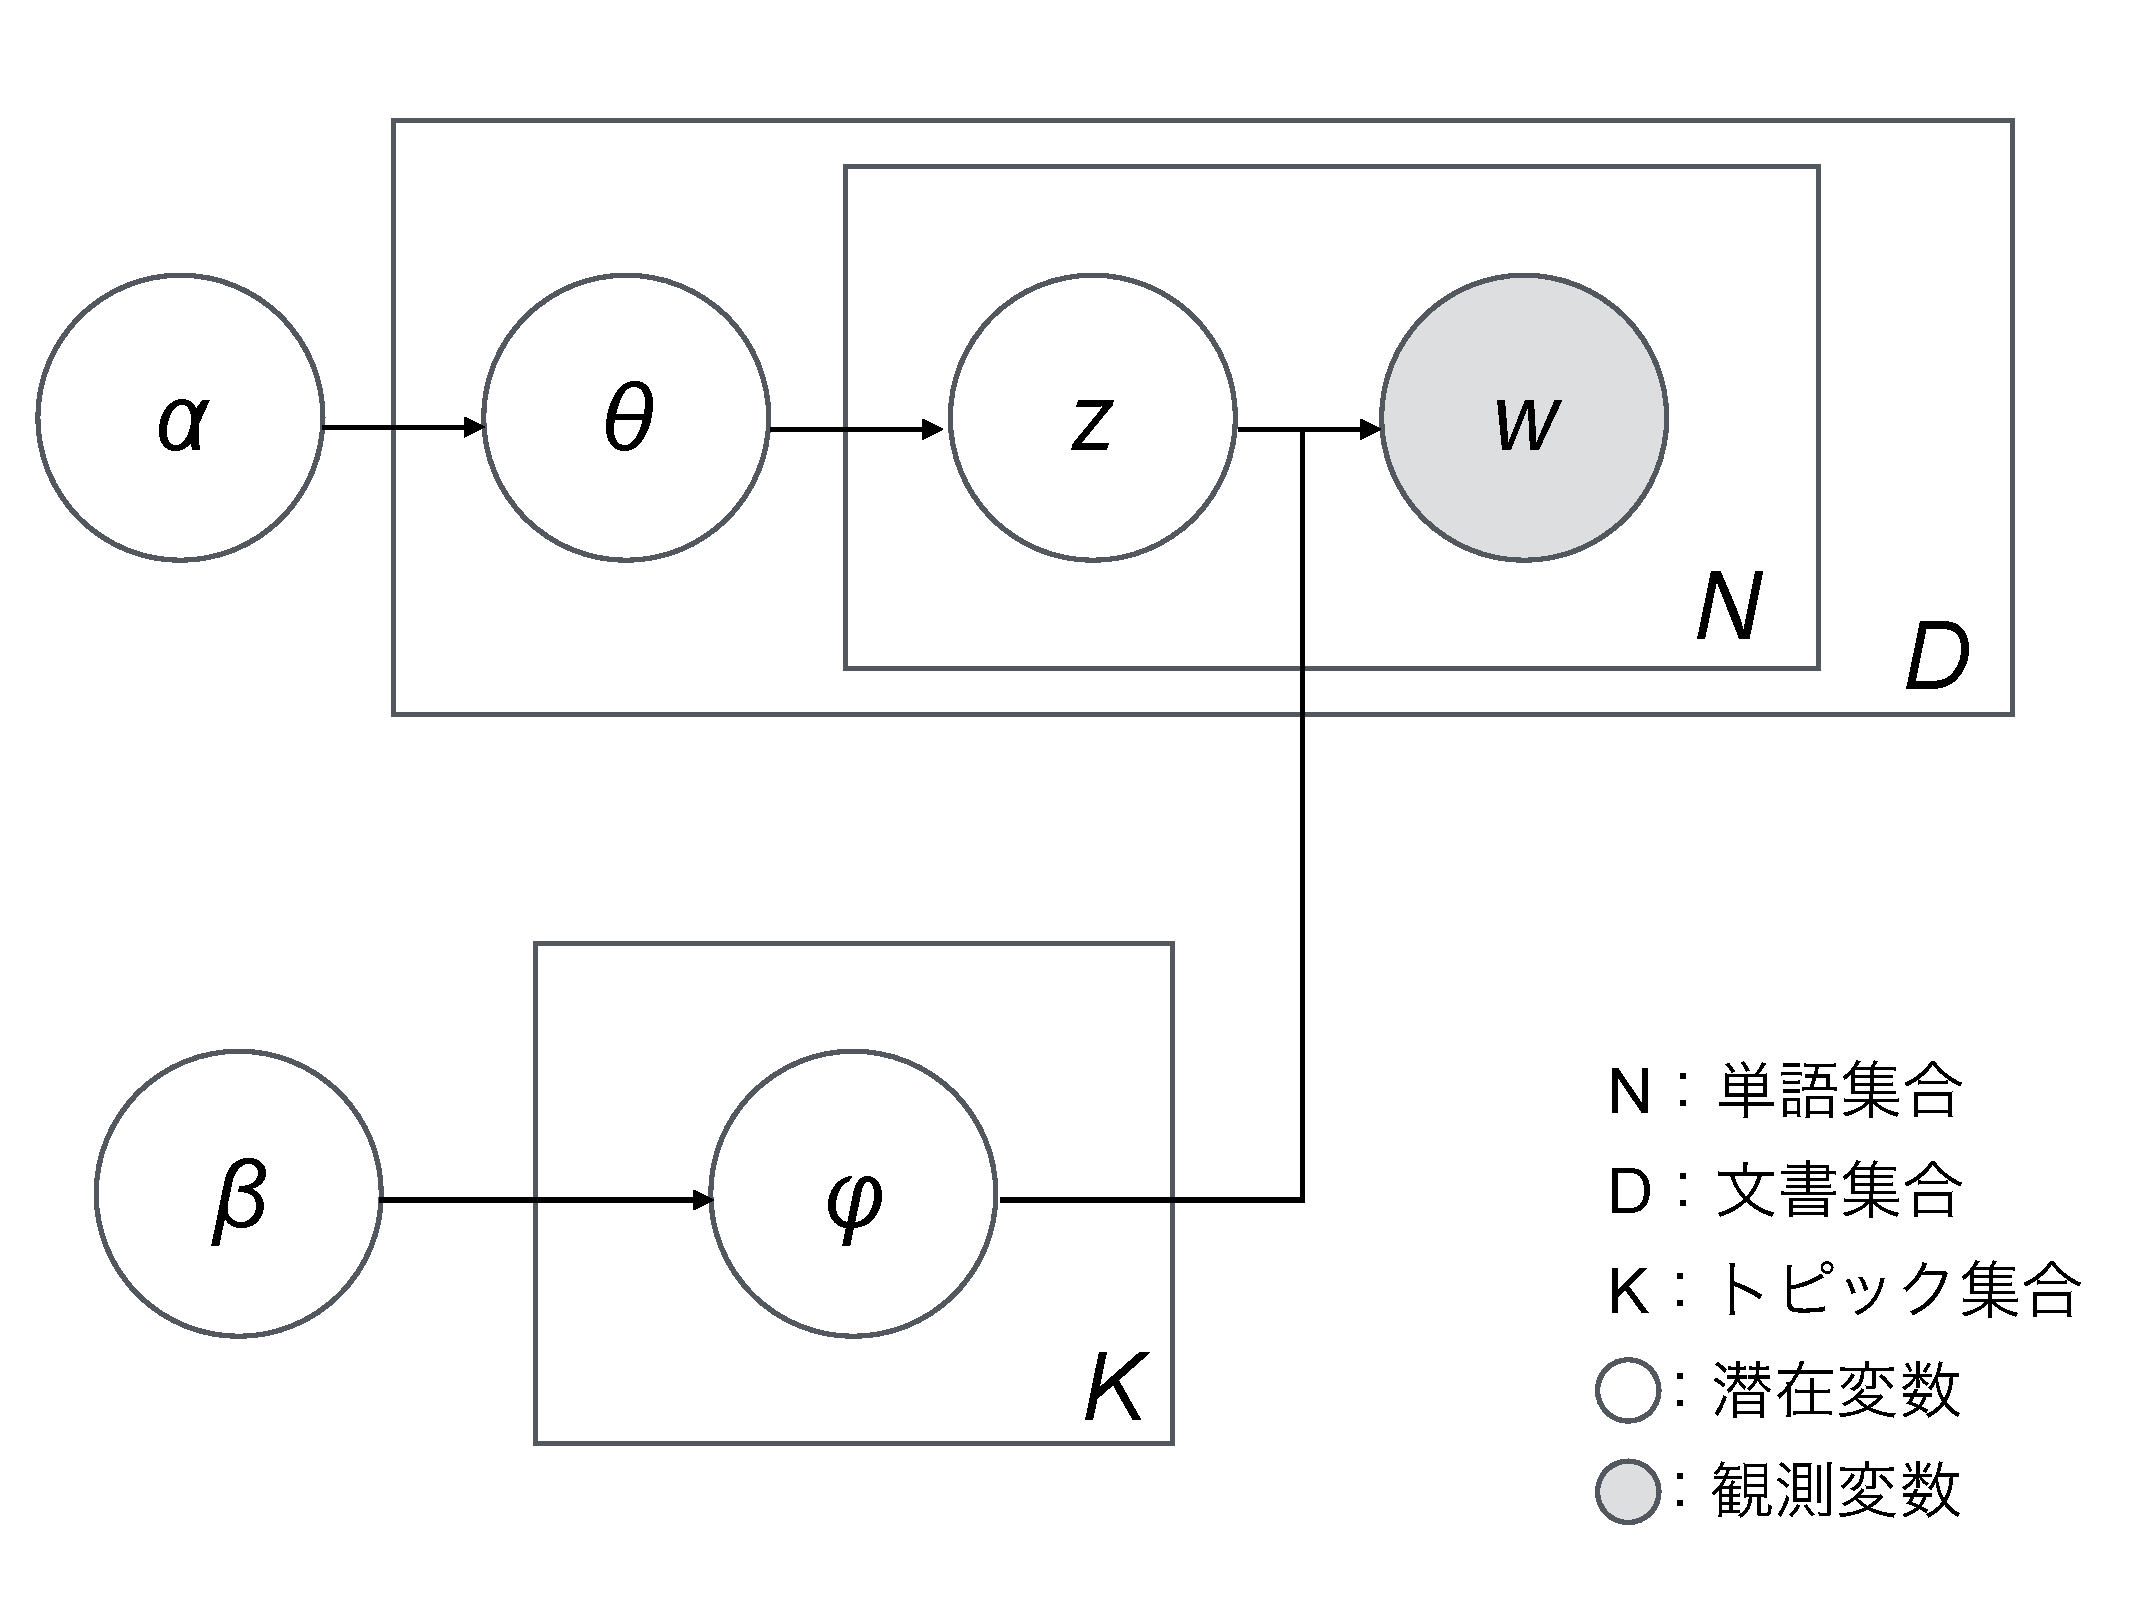
\includegraphics[width = 70mm]{figures/LDA.pdf} %貼り付ける画像と大きさ
	\end{center}
	\caption{LDAのグラフィカルモデル} %キャプション
	\label{fig:lda} %TEXコード内で使う変数指定
\end{figure}
トピック分布$\theta$と各トピックにおける単語分布$\phi$の推定には,GriffthsらのGibbs Samplingによる推定手法を用いた\cite{gibbs}.


\subsubsection{LDAによる評価観点の学習}
		\label{subsubsec:learning}
本節では,全ての書籍レビューに対してLDAを用いて,書籍を評価する際の多様な観点をトピックとして抽出する.このとき,書籍自体に関するトピックが抽出されるのは避けることが望ましい.そこで,書籍の登場人物名や作者名,など特定の書籍のみに出現するような単語を除外するために,以下の前処理を行う.
\par
全書籍のレビューを Mecab\cite{mecab}を用いて形態素解析し,名詞・形容詞・形容動詞を抽出する.そして,それぞれの書籍ごとに,その書籍に対する全レビュー中の単語$w$を含むレビューの割合を求める.形式的には,書籍$b$における単語$w$を含むレビューの出現率$\mathrm{r}(b,w)$を以下の式で表す.
\begin{equation}
\mathrm{r}(b,w) = \frac{ \mid\{r \mid r \in \mathrm{reviews}(b), w \in \mathrm{words}(r)\}\mid}{\mid \mathrm{reviews}(b) \mid }
\end{equation}
ここで,$\mathrm{reviews}(b)$は書籍$b$を含むレビュー集合であり,$\mathrm{words}(r)$はレビュー$r$を含む全単語からなる集合を表す.
書籍集合$B$における,それぞれの書籍に対する単語$w$の平均出現率が低い場合は,その単語は特定の書籍固有の単語であると考えられるため,評価観点要素の抽出には用いないこととする.書籍集合$B$における単語の$w$の一般度$\mathrm{major}(B,w)$を以下の式で定義する.
\begin{equation}
\mathrm{major}(B,w) = \frac{\sum_{b\in B}{\mathrm{r}(b,w)}}{\mid B \mid}
\end{equation}

上記の式によって,求められた一般度$major(B,w)$が設定した閾値より低い単語をトピック抽出の対象から除外する.一般度の低い単語が除外された,全レビュワーの全レビューに対してトピック抽出を行い,得られたトピックの集合を,書籍評価における観点トピックの集合とする.
抽出された書籍評価の観点トピックの例を表\ref{table:topic}に示す.ここで対象としたのは「読書メーター」に含まれる書籍レビューである.対象としたレビュワー数は9万5,719人であり,これらのレビュワーの投稿した全てのレビュー,計1233万1749件を用いた.トピック数は100とし,各トピックあたりに含まれる単語数は10と設定した.
\begin{table}[tb]
  \begin{center}
    \caption{観点トピックの例}
    \label{table:topic} %TEXコード内で使う変数指定
    \begin{tabular}{|l|l|l|l|} \hline
      topic1 & topic2 & topic3 & topic4 \\ \hline \hline
      キャラ & 自分 & 漫画 & 最後 \\
      主人公 & 子供 & 絵 & 登場人物 \\
      感じ & 本 & 作品 & 描写 \\
      これ & それ & 購入 & 印象 \\
      ヒロイン & 家族 & 表紙 & もの \\
      かわいい & ため & 先生 & ラスト \\
      期待 & 心 & 絵柄 & 物語 \\
      ラブコメ & 親 & 作者 & 伏線 \\
      設定 & 時代 & 楽しみ & 人間 \\
      漫画 & 気持ち & 連載 & 文章 \\ \hline
    \end{tabular}
  \end{center}
\end{table}

		\subsubsection{LDAによる評価観点の推論}
レビュワーの全レビューを一纏めにしたものを1つの新規文書として,LDAの推論計算により,観点トピックに対して,新規文書はどのトピックが生成しやすいかの多項分布$\theta_{d_{new}}$を以下の式で推定することができる.
\begin{equation}
\theta_{d_{new}} = \sum_{ z=1 }^{K}p(z)p(\mathbf{d}_{new}|z)
\end{equation}
$p(z)$は混合比と呼ばれ,トピック$z$が選ばれる確率を表し,\ref{subsubsec:learning}で学習したモデルでの全体における$\theta_{z}$に対応している.$p(\mathbf{d}_{new}|z)$はトピック$z$が選ばれたときに文書$\mathbf{d}_{new}$が生成される確率を表し,これに$p(z)$をかけることで,ベイズ推定より,文書$d_{new}$においてトピック$z$が選ばれる確率である$\theta_{d_{new},z}=p(z | \mathbf{d}_{new})$を求めている.これをレビュワーの評価観点ベクトルとして扱う.

	\section{レビュワーの信頼度を利用した協調フィルタリング}
		\subsection{既知のユーザに対する信頼度の推定}
\label{subsec:trust}
\ref{sec:feedback}で得られた評価情報に基づいて,対象ユーザが評価したユーザに対する信頼度を推定する.図\ref{fig:trust1}は,既知のユーザに対する信頼を推定するモデル図である.対象ユーザは既知のユーザが投稿した文書に対する評価を行う.しかし,一件のレビューからレビュワーを正しく評価できるとは限らないという問題がある.例えば,負の評価を入力されたレビューが普段のレビュワーらしくない文書だった場合,そのレビュワーの他のレビュー全てが対象ユーザにとって価値が低いとは言えない.本研究では,レビュワーの価値を計算する際に,評価された文書がどれだけそのユーザらしい発言であるかという確信度(Confidnece)を考慮する.レビューの確信度は,任意のレビューがレビュワーらしい文書である時に高くなり,レビュワーらしくない場合には低くなる値である.

\begin{figure}[tb]
	\begin{center} %貼り付ける位置指定
		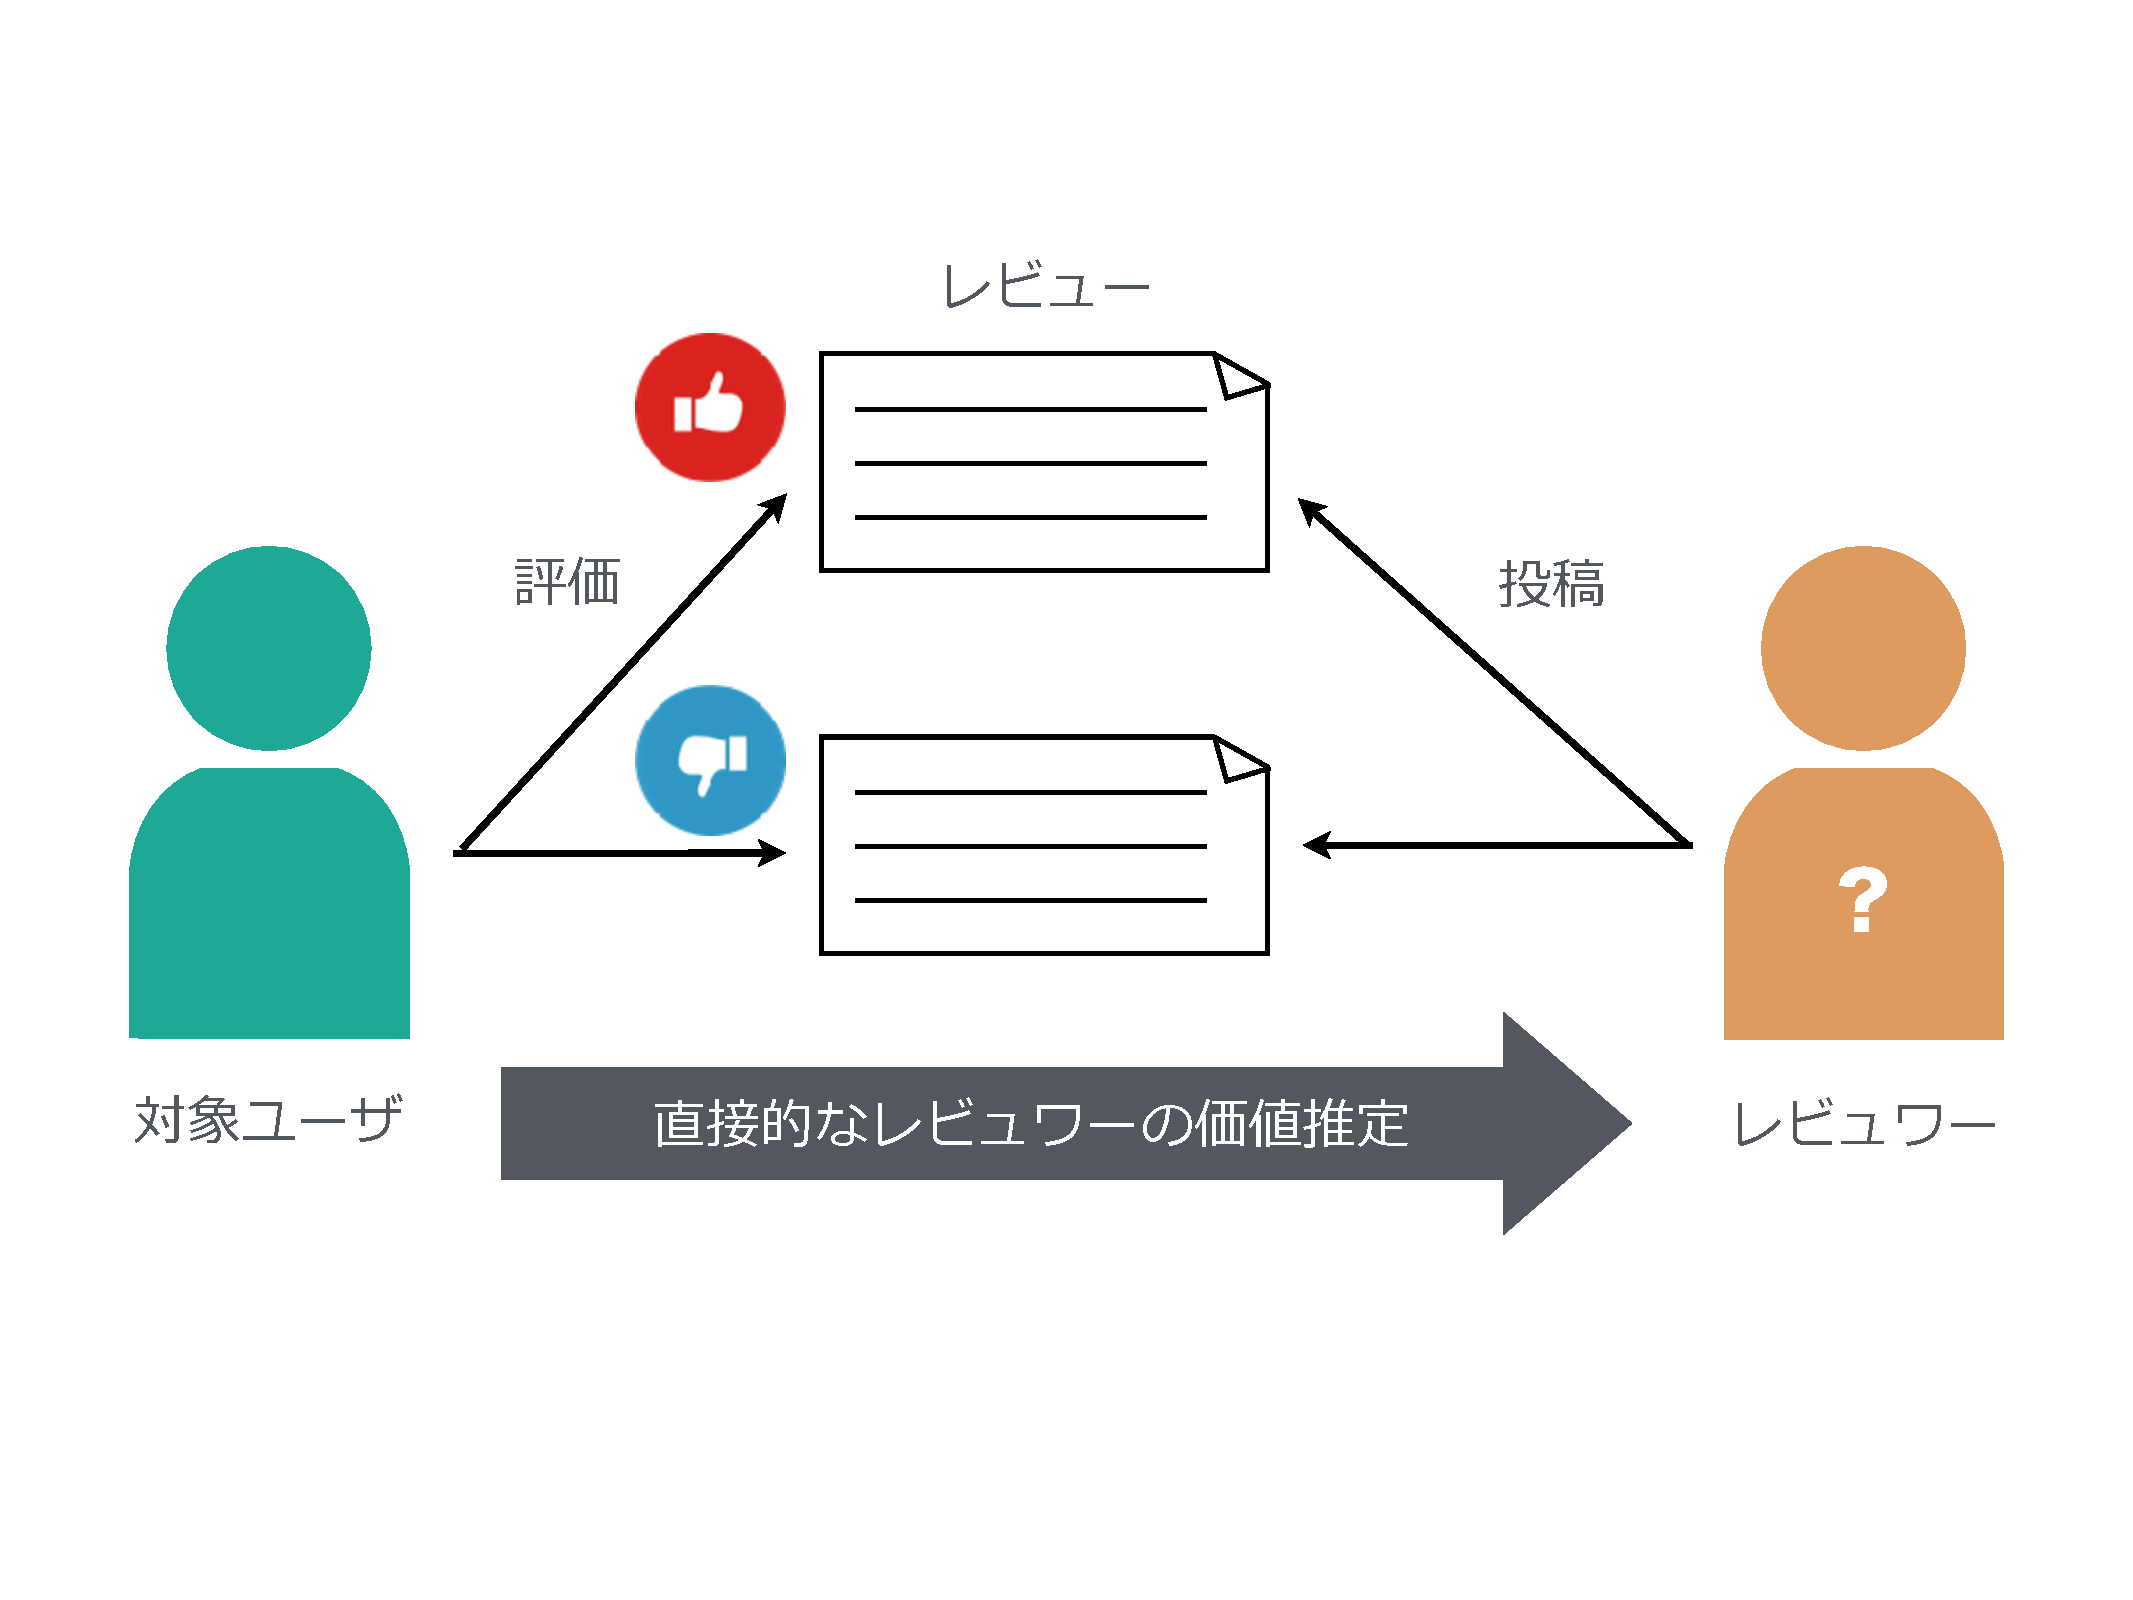
\includegraphics[width = 110mm]{figures/trust1.pdf} %貼り付ける画像と大きさ
	\end{center}
	\caption{評価されたユーザに対する信頼} %キャプション
	\label{fig:trust1} %TEXコード内で使う変数指定
\end{figure}
対象ユーザ$u$が評価したレビューを投稿したレビュワー$r$に対する信頼度$\mathrm{trust}(u, r)$は,評価に基づき,以下の式で定義する.
\begin{equation}
\mathrm{trust}(u ,r)=\frac{1}{\|D_r(pos)\|}\sum_{d\in{D_r(pos)}} \mathrm{conf}(d, r) - \frac{1}{\|D_r(neg)\|}\sum_{d\in{D_r(neg)}} \mathrm{conf}(d, r)
\end{equation}
この式では,対象ユーザからポジティブな評価を受けた文書集合の典型性の総和から,ネガティブな評価を受けた文書集合の典型性の総和を引くことにより,対象ユーザが既知であるユーザに対する信頼度を推定している.
ここで,$D_r(pos)$はレビュワー$r$の投稿した文書集合のうち,対象ユーザからポジティブな評価を受けた文書集合を表し,$D_r(neg)$はレビュワー$r$の投稿した文書集合のうち,対象ユーザからネガティブな評価を受けた文書集合を表し,$d$は1つの文書を表している.$\mathrm{conf}(d, r)$は文書$d$がどれだけレビュワー$r$らしい文書であるかについての確信度を表し,本研究では,$\mathrm{conf}(d, r)$をレビュワー$r$における文書$d$の確信度と定義する.確信度の詳細に関しては\ref{subsec:p}で後述する.


	\subsection{未知のユーザに対する信頼度の推定}
\label{subsubsec:weight}
ここでは,\ref{subsec:trust}で得られた既知のユーザに対する信頼情報に基づいて,対象ユーザがまだ評価していないユーザに対する信頼度を推定する手法について述べる.
\begin{figure}[tb]
	\begin{center} %貼り付ける位置指定
		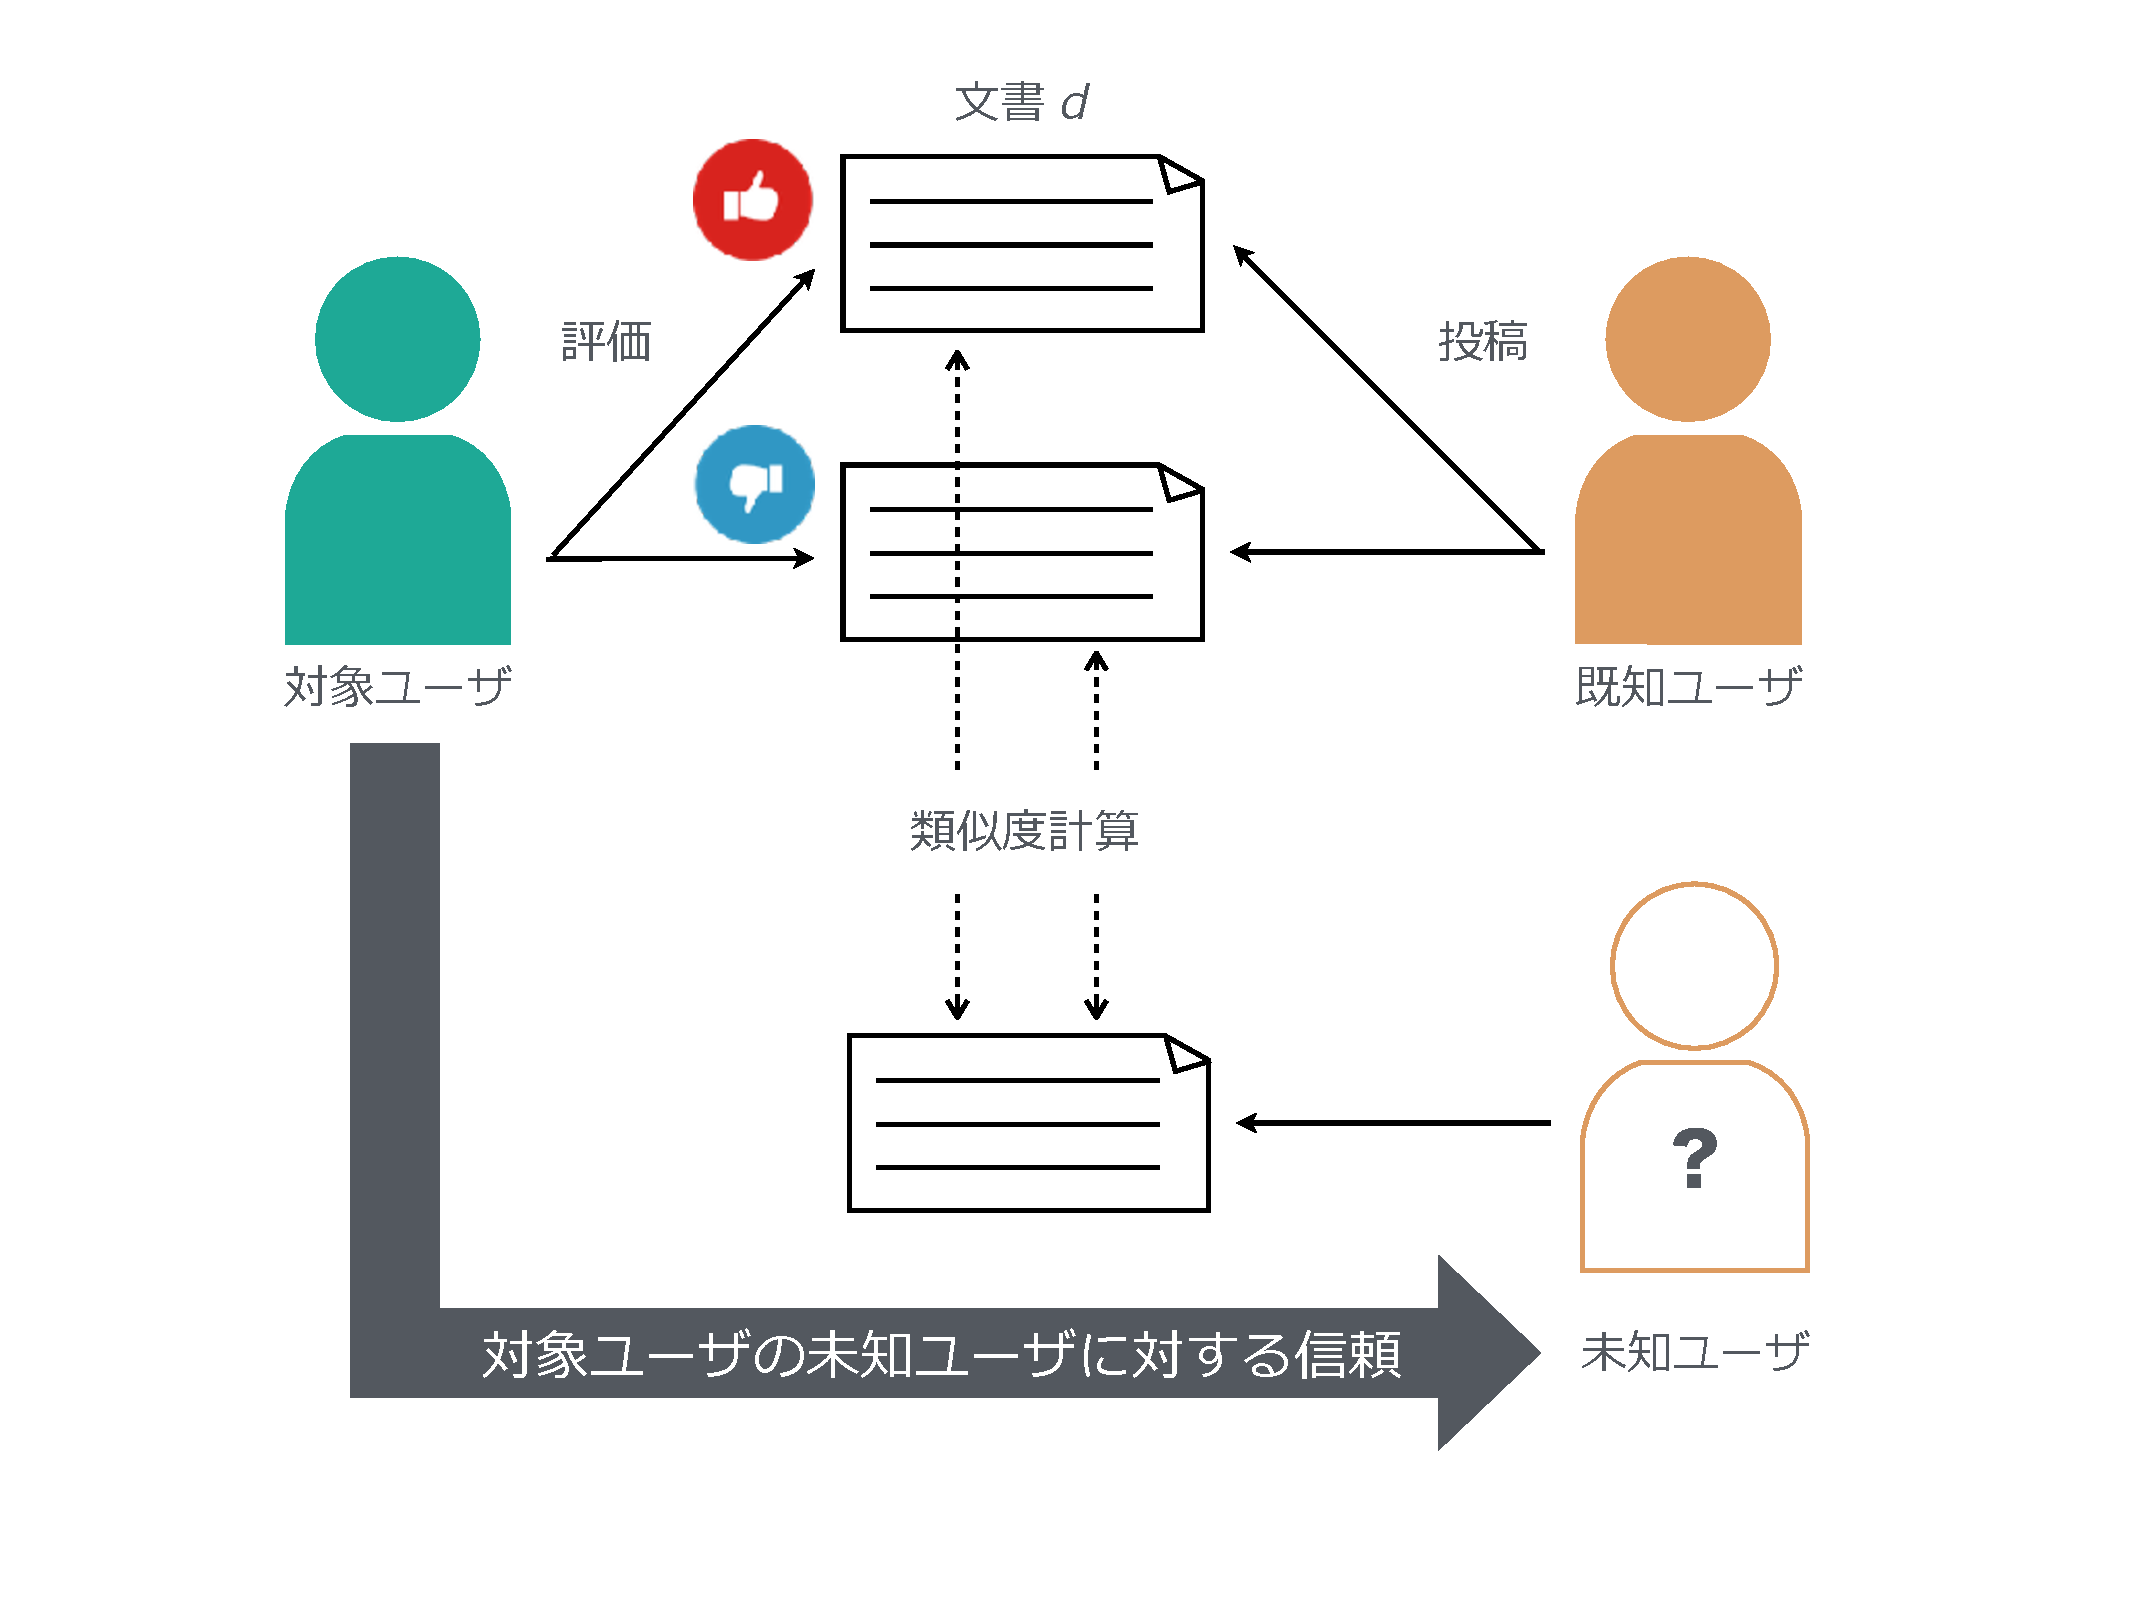
\includegraphics[width = 110mm]{figures/trust2.pdf} %貼り付ける画像と大きさ
	\end{center}
	\caption{未知のユーザに対する信頼} %キャプション
	\label{fig:trust2} %TEXコード内で使う変数指定
\end{figure}
本手法では,対象ユーザに評価されたユーザの特徴ベクトルと,まだ評価されていないユーザの特徴ベクトルとの間のコサイン類似度を求め,得られた値がまだ実際には評価されていないレビュワーに対する信頼度に影響を与える.信頼度の高いレビュワーと似ているレビュワーの価値は高く,反対に信頼度の低いレビュワーと似ているレビュワーの価値は低いという考えに基づいて,対象ユーザ$u$に対する任意のレビュワー$r$の信頼スコア$\mathrm{trust}(u, r)$は以下の式で計算される.
\begin{equation}
\begin{split}
\mathrm{trust}(u ,r) = &\bigl(\sum_{d\in{D(pos)}}\mathrm{sim}(d, d_{r})-\sum_{d\in{D(neg)}}\mathrm{sim}(d, d_{r})\bigr)\\
&\times\mathrm{conf}(d_{r}, r)
\end{split}
\end{equation}
この式では,対象ユーザからポジティブな評価を受けた文書集合と信頼を推定したい未知のユーザの文書との類似度の総和からネガティブな評価を受けた文書集合と信頼を推定したい未知のユーザの文書との類似度の総和を引き,得られた値に文書の典型性を掛け合わせることで,対象ユーザが未知であるレビュワーに対する信頼度を推定している.
ここで,$\mathbf{D}_{pos}$は対象ユーザからポジティブな評価を受けた文書集合,$\mathbf{D}_{neg}$は対象ユーザからネガティブな評価を受けた文書集合を表している.$\mathrm{sim}(d, d_{r})$は,文書$d$と未評価レビュワー$r$の文書$d_r$との間の類似度を表し,Doc2Vecによりベクトル化された$\mathbf{d}$と$\mathbf{d_r}$の間のコサイン類似度を計算することで求める.

	\subsection{文書の確信度について}
\label{subsec:p}
本研究では,評価された文書がどれだけそのユーザらしい発言であるかという確信度を信頼推定モデルの中に組み込むことで,計算される信頼度の確信性を向上させる.文書の確信度は,ユーザが今まで投稿した全ての文書をひとまとめにした文書のベクトルと,対象となる文書ベクトルとの間のコサイン類似度を計算することで求める.レビュワー$r$における文書$d$の確信度$\mathrm{conf}(d , r)$は以下の式で定義される.
\begin{equation}
\mathrm{conf}(d, r) = \mathrm{cos}\bigl(\mathbf{d}, \mathbf{D}_r\bigr)
\end{equation}
$\mathbf{d}$は典型性を求めたい文書のベクトルであり,$\mathbf{D}_r$はユーザ$u$が投稿した文書全体のベクトルである.文書のベクトル化はどちらもDoc2Vecを利用して行う.

\begin{figure}[tb]
	\begin{center} %貼り付ける位置指定
		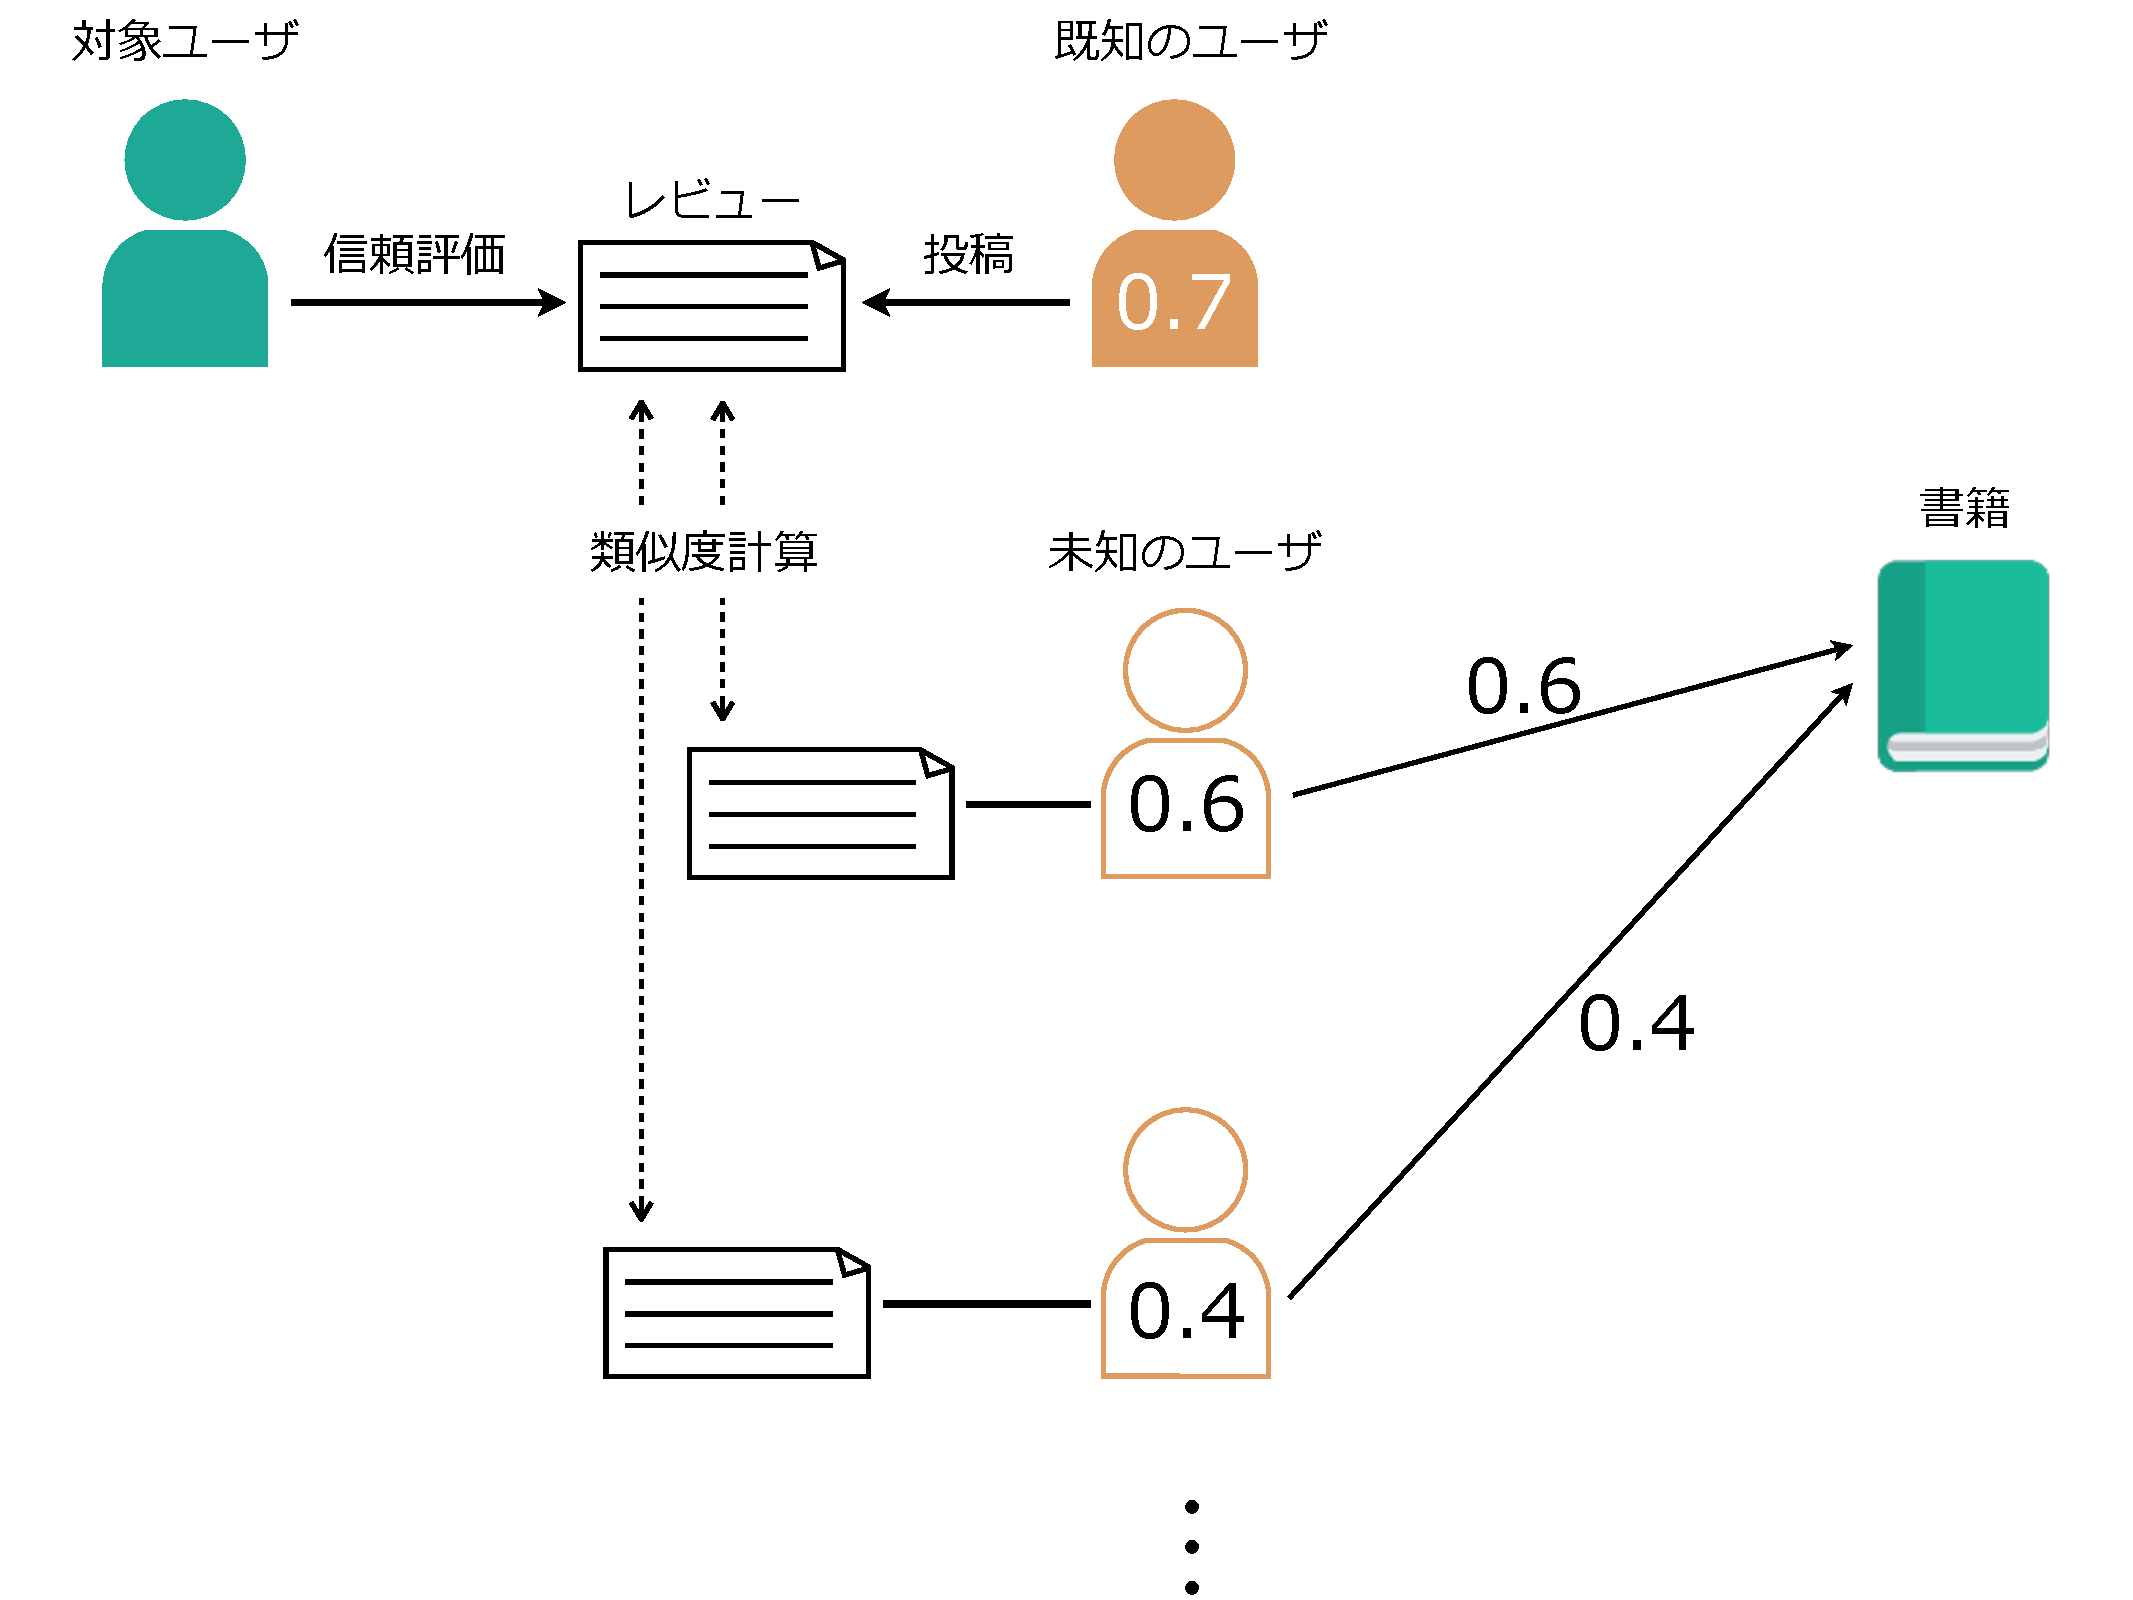
\includegraphics[width = 110mm]{figures/model.pdf} %貼り付ける画像と大きさ
	\end{center}
	
	
	\section{レビュワーの重みを利用した協調フィルタリングの拡張} %キャプション
	\label{fig:model} %TEXコード内で使う変数指定
\end{figure}
提案モデルに基づき,オンラインレビューサイトにおけるレビュワーに対する価値を推定し,その値をレビュワーに対する重みとして,推薦書籍の計算および提示を行う.
書籍$b_{1}$を選択した時の,ユーザ$u$に対する書籍$b_{2}$の予測評価値は,以下の式で求める.
\begin{equation}
\mathrm{Pred}( u, b_{1}, b_{2} ) = \sum_{r\in{\mathbf{R}(b_{1})}}\bigl({\mathrm{trust}( u , r )}\times {\mathrm{read}( r , b_{2} )}\bigr)
\end{equation}
ここで,$\mathbf{R}(b)$は書籍$b$に対してレビューを投稿したレビュワー集合を表し,$\mathrm{trust}(u,r)$は対象ユーザ$u$にとってのレビュワー$r$の信頼度を表す.また,$\mathrm{read}(r,b)$は,レビュワー$r$が書籍$b$を読んだかどうかによって値が決まる.
\begin{equation}
	\mathrm{read}(r,b) =\left\{ \begin{array}{ll}
		1 & \mbox{(読んだ)} \\
		0 & \mbox{(読んでいない)} \\
	\end{array} \right.
\end{equation}
書籍$b_{1}$を読んだレビュワー集合のうち,書籍$b_{2}$を読んだレビュワーの信頼度の合計値がユーザ$u$に対する書籍$b_{2}$の予測評価値となり,これにより,ユーザの信頼度を考慮した協調フィルタリングによる推薦を行う.
	\section{評価実験}
プロトタイプを用いた被験者実験を行い,提案手法の有効性を評価した.
		\subsection{実験環境}
オンライン書籍レビューサイト「読書メーター」\cite{bookmeter}に登録しているレビュワーのうち計9万5,719人のレビュー,全1233万1749件を対象として,Doc2Vecの学習を行った.日本語解析にはMeCabを用いて,辞書はmecab-ipadic-neologd\cite{mecabdic}を使用した.ユーザに提示するレビューは,読書メーターに投稿されているレビューを用いた.

		\subsection{評価手法}
対象とした被験者は20代の男女8人であった.被験者には,最近読んだ書籍の中から,自由に書籍を選んでもらい,その書籍のレビューに対して,評価のフィードバックを入力してもらった.評価については「このレビューを支持するか」という基準で「支持する」,「わからない」,「支持しない」の3段階の評価とし,「支持する」「支持しない」がそれぞれ10件以上入力されるまでを入力してもらった.
プロトタイプシステムを通して得られた推薦結果上位20件のうち,未読書籍について「あらすじ」と「レビュー」を読んでもらい,「その推薦書籍を読みたいと思うかどうか」に関して「思う」,「どちらかと言えば思う」,「どちらとも言えない」,「どちらかと言えば思わない」,「思わない」の5段階でアンケート調査を行った.書籍の「1巻」「2巻」などは,まとめてシリーズとしての評価を行った.ベースラインは,信頼度を均一に設定した協調フィルタリングによる推薦とした.また,文書の典型性を考慮することの有効性を評価するために,典型性を考慮しない場合の提案手法による推薦も行った.
		\subsection{実験結果}
\begin{figure}[tb]
	\begin{center} %貼り付ける位置指定
		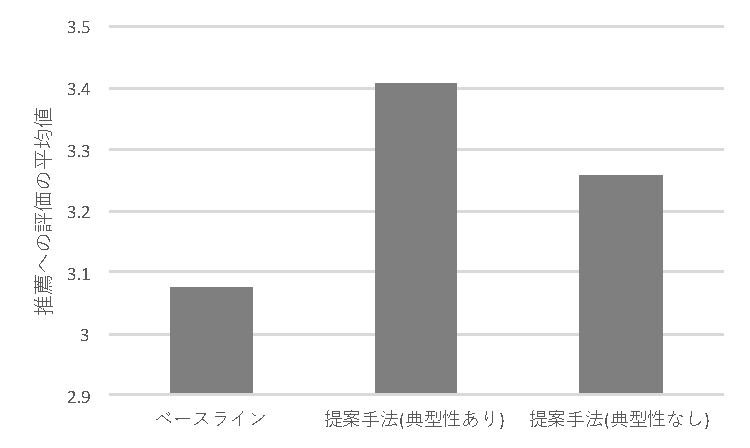
\includegraphics [width = 110mm] {figures/result2.pdf} %貼り付ける画像と大きさ
	\end{center}
	\caption{推薦書籍への平均評価値} %キャプション
	\label{fig:result1} %TEXコード内で使う変数指定
\end{figure}

\begin{figure}[tb]
	\begin{center} %貼り付ける位置指定
		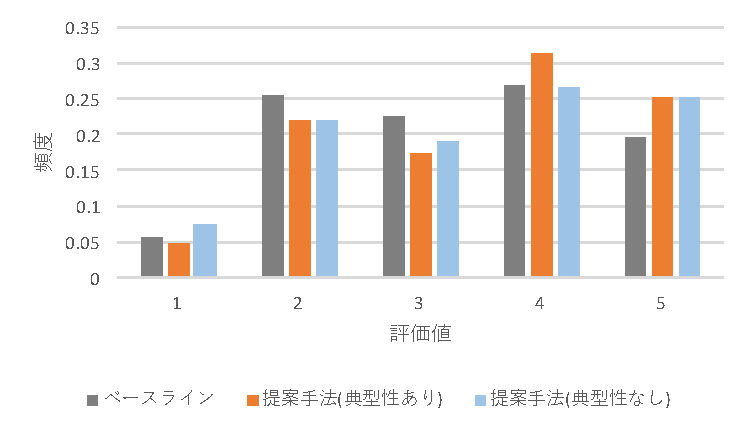
\includegraphics [width = 110mm] {figures/result.pdf} %貼り付ける画像と大きさ
	\end{center}
	\caption{評価値の頻度分布} %キャプション
	\label{fig:result2} %TEXコード内で使う変数指定
\end{figure}

「その推薦書籍を読みたいと思うかどうか」に関して「思う」,「どちらかと言えば思う」,「どちらとも言えない」,「どちらかと言えば思わない」,「思わない」の評価を,それぞれ5点,4点,3点,2点,1点として,手法ごとに,推薦書籍への評価の平均値を求めた.提案手法とベースラインのスコアを図\ref{fig:result1}に示す.縦軸は推薦書籍への評価の平均値であり,横軸は左からベースライン,提案手法(典型性あり),提案手法(典型性なし)である.また,評価値ごとの頻度分布を図\ref{fig:result2}に示す.
	\section{議論}
提案手法とベースラインとの間で,有意水準5%において有意な差が見られ,また,提案手法(典型性あり)はベースラインと比較して,評価値1〜3の頻度が低く,反対に評価値4〜5の頻度が高いことから,提案手法は書籍推薦の精度を上げるうえで有効であることが分かった.また,提案手法の中でも,典型性を考慮した手法としなかった手法を比較すると,典型性を考慮した手法の方が,考慮しなかった手法よりも,評価の平均値が高く,また評価値の頻度分布においても,評価値4の頻度が考慮しない手法より高く,評価値1〜3の頻度は低かった.このことから,文書の典型性を考慮することが信頼度推定の精度を向上させる上で有効であることがわかった.


\chapter{レビュワーの信頼度に基づくアイテムの品定め支援}
	\section{アイテムの品定めにおけるレビュー推薦の必要性}
アイテム推薦によって,検討候補のアイテムが絞り込まれた後,ユーザは対象のアイテムが本当に自分にとって価値のあるものであるのかについて品定めを行うことが考えられる.未知のアイテムの品定めをする際に,レビューはアイテムの使用感や微細な情報を得る上で非常に有用であり,株式会社情報通信総合研究所の調査\cite{ict}では,インターネットショッピングサービスを利用する際に,全体の74.8%の人がレビューを参考にすると回答している.しかし,現在オンラインレビューサイト上には莫大な数のレビューが存在し,効率的に有用なレビューを発見することは難しいという問題がある.また,投稿されているレビューは対象ユーザにとって役に立つレビューばかりではなく,中には対象ユーザにとって役に立たないレビューも存在する場合がある.

	\section{レビュワーの信頼度に基づくレビュー推薦手法}
コンテンツの品定めをする上で有用なレビューは,対象ユーザと感覚が近いレビュワーのレビューであると考えられる.そこで,ユーザの共感できるレビューを推定し,上位に表示することで、効率的な品定めを支援する.
\ref{subsec:trust}で得られたレビュワーに対する信頼値を基に,未知のアイテムのレビューの価値を推定する.信頼値の高いレビュワーと似ているレビュワーも信頼できるという仮定に基づいて,対象ユーザ$u$に対するレビュー$d$の推薦スコアは以下の式で計算される.
\begin{equation}
\begin{split}
\mathrm{score}(u ,d)=&\frac{\sum_{r\in{RVR(PR, NR)}} \mathrm{trust}(u,r) \times \mathrm{sim}(r, r_d)}{\sum_{r\in{RVR(PR, NR)}} \mathrm{sim}(r, r_d)}\\
&\times conf(d, r_d)
\end{split}
\end{equation}
ここで,$PR$はユーザ$u$の投稿した文書集合のうち,対象ユーザからポジティブな評価を受けた文書集合を表し,$NR$はユーザ$u$の投稿した文書集合のうち,対象ユーザからネガティブな評価を受けた文書集合を表す.$r_d$は文書$d$を投稿したレビュワーを表しており,\ref{subsec:trust}で推定したレビュワー$r$の信頼値に対して,レビュワー$r$とレビュワー$r_d$の類似度を掛け合わせ,重み付き平均を計算することで,レビュワー$r_d$の信頼値を推定し,得られた値に$conf(d, r_d)$を掛け合わせることで,ユーザ$u$に対する文書$d$の推薦スコアを計算している.レビュワー同士の類似性$\mathrm{sim}(r, r_d)$は,文章の分散表現を獲得できるDoc2Vec \cite{doc2vec} を用いて計算される.具体的には,レビュワーが投稿した文書を一纏めにした文書をDoc2Vecによってベクトル化し,ベクトル同士の類似度をコサイン類似度によって計算する.
レビュワー集合$RVR$は以下の式で決定される.
\begin{equation}
\mathrm{RVR}(PR ,NR)=\bigcup_{d\in{PR\cup NR}} \mathrm{reviewer}(\mathrm{item}(d))
\end{equation}
ここで,$\mathrm{item}(d)$は文書$d$が投稿されているアイテム集合を表し,$\mathrm{reviewer}(\mathrm{item}(d))$は文書$d$が投稿されているアイテム集合にレビューを投稿しているレビュワー集合を表している.

	\section{評価実験}
		\subsection{実験環境}
ユーザに提示するレビューおよび推薦に利用するアイテム評価データは,オンライン書籍レビューサイト「読書メーター」を用いた.日本語解析にはMeCab\cite{mecab}を用いて,辞書はmecab-ipadic-neologd\cite{mecabdic}を使用した.

		\subsection{評価手法}
被験者には,最近読んだ書籍の中から,自由に書籍を2冊選んでもらい,2冊の書籍のレビューに対して,評価のフィードバックを入力してもらう.評価については「このレビューに共感するか」という基準で「共感する」,「わからない」,「共感しない」の3段階の評価とし,それぞれ100件のレビューを評価してもらう.片方の書籍のレビューに対する評価データを学習データとして,もう一方の書籍のレビューに対する推薦スコアを予測する.
提案手法を通して得られた推薦結果上位10件に含まれる,「共感する」,「わからない」,「共感しない」の割合を算出した.ベースラインは,読書メーターに設置されているレビューに対する投票数の高い順に並び替えたレビューとする.
	\section{議論}

\chapter{まとめ}

%%%% 謝辞
\chapter*{謝辞}
\addcontentsline{toc}{chapter}{謝辞}
三年間,本研究に際して,熱心なご指導をいただきました牛尼剛聡准教授に心から感謝いたします.
\par
また,様々なアドバイスをいただきました牛尼研究室の皆様,本当にありがとうございました.

%%% 参考文献はここに
\begin{thebibliography}{99}
	%はじめに
	\bibitem{rakuten}楽天市場, http://www.rakuten.co.jp
	\bibitem{rakuten_info}http://www.rakuten.co.jp/com/inc/rc/info.html
	\bibitem{google}“Google Books:Books of the world, stand up and be counted! All 129,864,880 of you.”,
	\par
	http://booksearch.blogspot.jp/2010/08/books-of-world-stand-up-and-be-counted.html, (2017/01/22アクセス)
	\bibitem{info}Christopher D. Manning, Prabhakar Raghavan, Hinrich Schutze,“Introduction to Information Retrieval”, Cambridge University Press, 2008.
	\bibitem{@cosme}@cosme, http://www.cosme.net/
	\bibitem{bookmeter}読書メーター, http://bookmeter.com/
	\bibitem{yahoo}Yahoo!映画, http://movies.yahoo.co.jp/
	
	%関連研究
	\bibitem{hijikata2}土方 嘉徳, “利用者の好みをとらえ活かす-嗜好抽出技術の最前線- : 1.嗜好抽出・情報推薦の基礎理論 1)嗜好抽出と情報推薦技術”, 情報処理, Vol.48, No.9, pp.957-965, 2007.
	%適合フィードバック
	\bibitem{feedback}Foltz, P.W.: Using Latent Semantic Indexing for Information Filtering, Proc. of ACM Conference on Office Inforamtion Systems, pp.40-47, 1990.
	\bibitem{hijikata}土方 嘉徳, “情報推薦・情報フィルタリングのためのユーザプロファイリング技術,” 人工知能学会誌, vol.19, no.3, pp.365-374, 2004.
	\bibitem{yan}顔 洪, 牛尼 剛聡, “スマートフォンでの効率的な商品選別を目的としたユーザの振舞いに基づく閲覧リスト最適化手法”, 情報処理学会論文誌データベース(TOD),Vol.8, No.4, pp.1-15, 2015.
	%レビューを利用した情報推薦
	\bibitem{Li}Li Chen, Guanliang Chen, Feng Wang, Recommender systems based on user reviews: the state of the art. User Modeling and User-Adapted Interaction, June 2015, Vol. 25, pp 99-154
	\bibitem{hayashi}林 貴宏, 尾内 理紀夫, 「Web上のレビューを利用した映画推薦システム」, 人工知能学会論文誌
Vol.30, No. 1, pp.102-111, 2015.
	\bibitem{amazon}A Statistical Analysis of 1.2 Million Amazon Reviews: http://minimaxir.com/2014/06/reviewing-reviews
        \bibitem{Moghaddam}S. Moghaddam, M. Jamali, and M. Ester. ETF: Extended Tensor Factorization model for personalizing prediction of review helpfulness. In Procs. of the WSDM, Seattle, WA, USA, 2012. 
	\bibitem{Raghavan}Raghavan, S., Gunasekar, S., Ghosh, J.:Review quality aware collaborative filtering. In: Proceedings of the 6th ACM Conference on Recommender systems, pp. 123-130, 2012.
	%レビューランキング手法
	\bibitem{iki}伊木 淳, 亀井 清華, 藤田 聡, “レビューを対象とした信頼性判断支援システムの提案”, 情報処理学会論文誌, Vol.55, No.11, pp.2461-2475, 2014.
	\bibitem{muk}Mukherjee, A., Liu, B. and Glance, N.: Spotting Fake Reviewer Groups in Consumer Reviews, Proc. 21st International Conference on World Wide Web, pp.191-200 2012.
	\bibitem{xie}Xie, S., Wang, G., Lin, S. and Yu, P.S.: Review SpamDetection via Temporal Pattern Discovery, Proc. 18th ACM SIGKDD International Conference on Knowledge Discovery and Data Mining, pp.823-831, 2012.
	\bibitem{wang}Wang, G., Xie, S., Liu, B. and Yu, S.: Review Graph based Online Store Review Spammer Detection, Proc. 11th IEEE International Conference on Data Mining, pp.1242-1247, 2011.
	
	
	\bibitem{Blei}David M Blei, Andrew Y Ng, and Michael I Jordan. “Latent dirichlet allocation”, the Journal of machine Learn-ing research, Vol. 3, pp. 993-1022, 2003.
	
	%協調フィルタリング
	\bibitem{MF}Koren, Y., Bell, R. and Volinsky, C.: Matrix factorization techniques for recommender systems, Computer 42(8), pp.30-37 ,2009.
	\bibitem{Melville}Melville, P., Mooney, R. J. and Nagarajan, R.: Content boosted collaborative filtering for improved recommen- dations, Proc. AAAI, pp.187-192, 2002.
	\bibitem{CTR}Wang, C. and Blei, D.M.: Collaborative topic modeling for recommending scientific articles, Proc. ACM SIGKDD, pp.448-456, 2011.
	\bibitem{grouplens}Resnick, P., Iacovou, N., Suchak, M., Bergstrom, P. and Riedl, J.: GrxfoupLens: An Open Architecture for Collaborative Filtering of Netnews, Proc. ACM Conf. on Computer Supported Cooperative Work (CSCW’94 ), North Carolina, pp.175-186, 1994.
	
	%手法
	\bibitem{gibbs}Thomas L. Griffiths, Mark Steyvers : Finding Scientific Topics, Proc. National Academy of Sciences, vol.101, pp.5228-5235, 2004.
	\bibitem{word2vec}Tomas Mikolov, Greg Corrado, Kai Chen, and Jeffrey Dean. Efficient Estimation of Word Representations in Vector Space. In Proceedings of the International Conference on Learning Representations (ICLR 2013), pp.1-12, 2013.
	\bibitem{doc2vec}Quoc V, Leand Tomas Mikolov. DistributedRepresentations of Sentences and Documents, In Proceedings of The 31st In- ternational Conference on Machine Learning, pp. 1188-1196, 2014.	
	\bibitem{mecab}http://mecab.sourceforge.net/
	\bibitem{mecabdic}https://github.com/neologd/mecab-ipadic-neologd/blob/
	\par master/README.ja.md
	\bibitem{mecab}http://mecab.sourceforge.net/
	\bibitem{mecabdic}https://github.com/neologd/mecab-ipadic-neologd/blob/master/README.ja.md
	\bibitem{ict}"GDPに現れないICTの社会的厚生への貢献に関する調査研究", http://www.soumu.go.jp/johotsusintokei/linkdata/h28\_04\_houkoku.pdf
	
	
\end{thebibliography}

\chapter*{業績一覧}


\end{document}
